%%%%%%%%%%%%%%%%%%%%%%%%%%%%%%%%%%%%%%%%%
% Masters/Doctoral Thesis 
% LaTeX Template
% Version 2.5 (27/8/17)
%
% This template was downloaded from:
% http://www.LaTeXTemplates.com
%
% Version 2.x major modifications by:
% Vel (vel@latextemplates.com)
%
% This template is based on a template by:
% Steve Gunn (http://users.ecs.soton.ac.uk/srg/softwaretools/document/templates/)
% Sunil Patel (http://www.sunilpatel.co.uk/thesis-template/)
%
% Template license:
% CC BY-NC-SA 3.0 (http://creativecommons.org/licenses/by-nc-sa/3.0/)
%
%%%%%%%%%%%%%%%%%%%%%%%%%%%%%%%%%%%%%%%%%

%----------------------------------------------------------------------------------------
%	PACKAGES AND OTHER DOCUMENT CONFIGURATIONS
%----------------------------------------------------------------------------------------

\documentclass[
12pt, % The default document font size, options: 10pt, 11pt, 12pt
%oneside, % Two side (alternating margins) for binding by default, uncomment to switch to one side
oneside,
english, % ngerman for German
singlespacing, % Single line spacing, alternatives: onehalfspacing or doublespacing
%draft, % Uncomment to enable draft mode (no pictures, no links, overfull hboxes indicated)
%nolistspacing, % If the document is onehalfspacing or doublespacing, uncomment this to set spacing in lists to single
%liststotoc, % Uncomment to add the list of figures/tables/etc to the table of contents
%toctotoc, % Uncomment to add the main table of contents to the table of contents
%parskip, % Uncomment to add space between paragraphs
%nohyperref, % Uncomment to not load the hyperref package
headsepline, % Uncomment to get a line under the header
%chapterinoneline, % Uncomment to place the chapter title next to the number on one line
%consistentlayout, % Uncomment to change the layout of the declaration, abstract and acknowledgements pages to match the default layout
]{MastersDoctoralThesis}% The class file specifying the document structure%

\usepackage{polyglossia}
\usepackage{amsmath,amssymb,amsfonts}

\setmainlanguage{english}
\setotherlanguage{hindi}

\newfontfamily\devanagarifont[Script=Devanagari]{Noto Serif Devanagari}
\linespread{1.25}

\usepackage[utf8]{inputenc} % Required for inputting international characters
\usepackage[T1]{fontenc} % Output font encoding for international characters

\usepackage{mathpazo} % Use the Palatino font by default

\usepackage[backend=bibtex,style=ieee,natbib=true]{biblatex} % Use the bibtex backend with the authoryear citation style (which resembles APA)

\addbibresource{Bibliography.bib} % The filename of the bibliography

\usepackage[autostyle=true]{csquotes} % Required to generate language-dependent quotes in the bibliography

\usepackage{graphicx}
\usepackage{multirow}
\usepackage[normalem]{ulem}
\useunder{\uline}{\ul}{}
\usepackage{lscape}
\usepackage{mathrsfs}
\usepackage{longtable}
\usepackage{booktabs, tabularx}
\usepackage{float}
\usepackage{subfigure}
\usepackage{amsthm}
\usepackage{amssymb}
\usepackage{enumitem}
\usepackage{lipsum}
\usepackage{blindtext}
% \usepackage{subcaption}
% \usepackage{pdflscape}
% \usepackage{afterpage}

\usepackage[linesnumbered, ruled, vlined]{algorithm2e}
\usepackage[colorlinks]{hyperref}
\usepackage[noabbrev,  nameinlink]{cleveref}

\theoremstyle{definition}
\newtheorem{definition}{Definition}[section]

\theoremstyle{remark}
\newtheorem*{remark}{Remark}

%%%Author macros
\def\tsc#1{\csdef{#1}{\textsc{\lowercase{#1}}\xspace}}
\tsc{WGM}
\tsc{QE}
%%%



% Redefine the label format for equations
\crefformat{equation}{#2Equation~#1#3}
\Crefformat{equation}{#2Equation~#1#3}
%----------------------------------------------------------------------------------------
%	MARGIN SETTINGS
%----------------------------------------------------------------------------------------
\geometry{
	paper=a4paper, % Change to letterpaper for US letter
	inner=2.5cm, % Inner margin
	outer=2.5cm, % Outer margin
	bindingoffset=.5cm, % Binding offset
	top=1.5cm, % Top margin
	bottom=2.2cm, % Bottom margin
	%showframe, % Uncomment to show how the type block is set on the page
}

%----------------------------------------------------------------------------------------
%	THESIS INFORMATION
%----------------------------------------------------------------------------------------

\thesistitle{report title} % Your thesis title, this is used in the title and abstract, print it elsewhere with \ttitle
\supervisor{Dr. Vipin Kumar} % Your supervisor's name, this is used in the title page, print it elsewhere with \supname
\examiner{} % Your examiner's name, this is not currently used anywhere in the template, print it elsewhere with \examname
\degree{\uppercase{\textbf{Master of Techonolgy}}} % Your degree name, this is used in the title page and abstract, print it elsewhere with \degreename
\author{Subham Kumar\\ (MGCU2021CSIT4029)} % Your name, this is used in the title page and abstract, print it elsewhere with \authorname
\addresses{} % Your address, this is not currently used anywhere in the template, print it elsewhere with \addressname

\subject{Computer Science \& Engineering} % Your subject area, this is not currently used anywhere in the template, print it elsewhere with \subjectname
\keywords{} % Keywords for your thesis, this is not currently used anywhere in the template, print it elsewhere with \keywordnames
\university{\href{https://mgcub.ac.in}{Mahatma Gandhi Central University, Motihari, Bihar-845401, India}} % Your university's name and URL, this is used in the title page and abstract, print it elsewhere with \univname
\department{\href{https://mgcub.ac.in/department_of_computer_science.php}{DEPARTMENT OF COMPUTER SCIENCE AND INFORMATION TECHNOLOGY}} % Your department's name and URL, this is used in the title page and abstract, print it elsewhere with \deptname
\group{\href{http://researchgroup.university.com}{Research Group Name}} % Your research group's name and URL, this is used in the title page, print it elsewhere with \groupname
\faculty{\href{https://mgcub.ac.in/department_of_computer_science_faculty.php}{Dr. Vipin Kumar}} % Your faculty's name and URL, this is used in the title page and abstract, print it elsewhere with \facname

\AtBeginDocument{
\hypersetup{pdftitle=\ttitle} % Set the PDF's title to your title
\hypersetup{pdfauthor=\authorname} % Set the PDF's author to your name
\hypersetup{pdfkeywords=\keywordnames} % Set the PDF's keywords to your keywords
}
\usepackage{Edit}
\usepackage{ragged2e}
\usepackage{lscape}
 \usepackage{booktabs}
 \usepackage{graphicx}
 \usepackage{float}




\justifying
\begin{document}

\frontmatter % Use roman page numbering style (i, ii, iii, iv...) for the pre-content pages

\pagestyle{plain} % Default to the plain heading style until the thesis style is called for the body content


%--------------------cover----------------------
%----------------------------------------------------------------------------------------
%	COVER PAGE
%----------------------------------------------------------------------------------------

\begin{titlepage}
\begin{center}

%\vspace*{.06\textheight}

%\textsc{\Large Masters Thesis}\\[0.5cm] % Thesis type

%\HRule \\[0.4cm] % Horizontal line
{\LARGE \bfseries \ReportTitel \par}\vspace{0.3cm} % Thesis title
%\HRule \\[1.5cm] % Horizontal line

%\begin{minipage}[t]{0.4\textwidth}
%\begin{flushleft} \large
%%\emph{Author:}\\
%%\href{http://www.johnsmith.com}{\authorname} % Author name - remove the \href bracket to remove the link
%\end{flushleft}
%\end{minipage}
%\begin{minipage}[t]{0.4\textwidth}
%\begin{flushright} \large
%%\emph{Supervisor:} \\
%%\href{http://www.jamessmith.com}{\supname} % Supervisor name - remove the \href bracket to remove the link
%\end{flushright}
%\end{minipage}\\[1cm]
%
\vfill

\large \textit{A \rType  submitted to the \Uni}\\[0cm] % University requirement text
\large \textit{in partially fulfillment of the requirements}\\[0cm]
\large \textit{for the award of the degree of}\\[0cm]

\textbf{\Degree}\\[0cm]

\uppercase{In}\\[0cm]

\uppercase{\textbf{\Cour}}\\[0cm]

\uppercase{By}\\[0cm]

\uppercase{\textbf{\fAuthorC}}\\[1cm]




%   \begin{figure}[H]
        %   \centering
\centerline{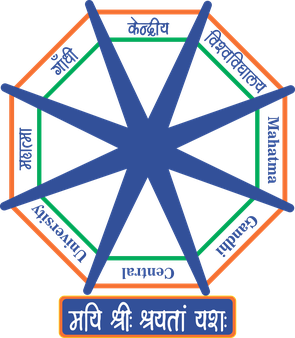
\includegraphics[height=1.5in,width=1.5in, keepaspectratio]{mgcu.png}}
        %   
\includegraphics{logo}% logo
    %   \end{figure}
\vfill
\vspace{1cm}
\normalsize{\departmentC}\\[-0.1cm] %search group name and department name
%\school\\[0.1cm]
%\large{\groupname}\\[-0.2cm]

{\scshape\Large \UniversityC \par}\vspace{1cm} % University name%\university\\[2cm]
\vfill

{\large \today}\\[1cm] % Date
%\includegraphics{Logo} % University/department logo - uncomment to place it

\vfill

\end{center}
\end{titlepage}
%--------------------cover----------------------

%--------------------Title----------------------
\begin{titlepage}
\begin{center}

%\vspace*{.06\textheight}

%\textsc{\Large Masters Thesis}\\[0.5cm] % Thesis type

%\HRule \\[0.4cm] % Horizontal line
{\LARGE \bfseries \ReportTitel \par}\vspace{0.1cm} % Thesis title
%\HRule \\[1.5cm] % Horizontal line

%\begin{minipage}[t]{0.4\textwidth}
%\begin{flushleft} \large
%%\emph{Author:}\\
%%\href{http://www.johnsmith.com}{\authorname} % Author name - remove the \href bracket to remove the link
%\end{flushleft}
%\end{minipage}
%\begin{minipage}[t]{0.4\textwidth}
%\begin{flushright} \large
%%\emph{Supervisor:} \\
%%\href{http://www.jamessmith.com}{\supname} % Supervisor name - remove the \href bracket to remove the link
%\end{flushright}
%\end{minipage}\\[1cm]
%
\vfill

\large \textit{A \rType submitted to the \Uni}\\[0cm] % University requirement text
\large \textit{in partially fulfillment of the requirements}\\[0cm]
\large \textit{for the award of the degree of}\\[0cm]

\textbf{\Degree}\\[0cm]

\uppercase{In}\\[0cm]

\uppercase{\textbf{\Cour}}\\[0cm]

\uppercase{By}\\[0cm]

\uppercase{\textbf{\fAuthorC \\[0cm] (\fAID)}}\\[0cm]

\large \textit{Under the Supervision of}\\[0cm]
\uppercase{\textbf{\SupervisorC}}\\[0.3cm]




%   \begin{figure}[H]
        %   \centering
        \centerline{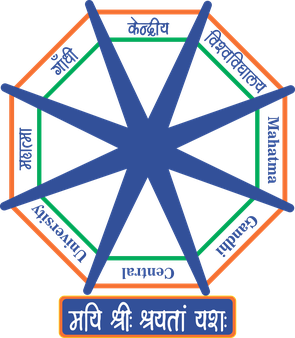
\includegraphics[height=1.5in,width=1.5in, keepaspectratio]{mgcu.png}}
        %   
\includegraphics{logo}% logo
    %   \end{figure}
\vfill
\vspace{0.3cm}
\normalsize{\departmentC}\\[-0.1cm] % Research group name and department name
%\school\\[0.01cm]
%\large{\groupname}\\[-0.2cm]

{\scshape\Large \UniversityC \par}\vspace{1cm} % University name%\university\\[2cm]
\vfill

{\large \today}\\[0.1cm] % Date
%\includegraphics{Logo} % University/department logo - uncomment to place it

\vfill
\end{center}
\end{titlepage}

%--------------------Title----------------------
%------------------------declaration------------
%----------------------------------------------------------------------------------------
%	DECLARATION PAGE
%----------------------------------------------------------------------------------------

\chapter*{}
\vspace*{-3.5cm}
% \thispagestyle{empty}

\setlength\tabcolsep{0pt}
\def\arraystretch{0}
\begin{table}[h]
\begin{center}
\begin{tabular}{r  l}
   \begin{minipage}{0.18\textwidth}
\begin{flushleft}
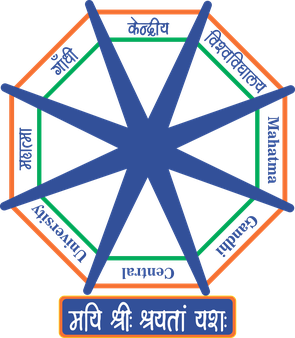
\includegraphics[height=1.25in,width=1.25in, keepaspectratio]{mgcu.png}
\end{flushleft}
\end{minipage}
&
\begin{minipage}{0.83\textwidth}
\begin{flushleft}

\begin{hindi}\Large \centering \departmentH\\
\end{hindi}
\centering\textbf{\department}\\
%\deptname\\[0.01cm] % Research group name and department name
\begin{hindi}\LARGE\centering\textbf{\UniversityH}\\
\end{hindi}
\vspace*{-0.1cm}
{\scshape\large\textbf\centering\UniversityC\par} % University name%\university\\[2cm]
\end{flushleft}
\end{minipage}
\noindent
\\
\end{tabular}
%\label{tab1}
\end{center}
\end{table}


\vspace{1.3ex}
\addchaptertocentry{\authorshipname} % Add the certificatename to the table of contents
\begin{center}
    \textbf{\LARGE\underline {DECLARATION}}
\end{center}

\vspace{3ex}
This is to certify that the \rType entitled {\bfseries " \ReportTitel "} is being submitted to the
\textbf{\department, \University } in partial fulfillment of
the requirements for the award of the degree of \textbf{\fACourse} in \textbf {Computer Science \& Engineering}, is a record of bonafide work carried out by me under the
supervision of  \textbf{"\Supervisor, \department, \University ."}\\[0.1cm]
\indent The matter embodied in the dissertation has not been submitted in part or full to any
University or Institution for the award of any other degree or diploma.
\par During the preparation of this work, I have not used any AI-based tool to write any part of this dissertation report. I take full responsibility for the submitted content including similarity.
\vspace*{0.3cm}

\setlength\tabcolsep{0pt}
\def\arraystretch{0}
\begin{table}[h]
\begin{center}
\begin{tabular}{r  r}
   \begin{minipage}{0.4\textwidth}
\begin{flushleft}

\end{flushleft}
\end{minipage}
&
\begin{minipage}{0.6\textwidth}
\begin{flushleft}

\vspace*{0.1cm}

\textbf \Author

\department\\[.1cm]
\University\\[.1cm]
Email id: - \fAemail
\end{flushleft}
\end{minipage}
\noindent
\\
\end{tabular}
%\label{tab1}
\end{center}
\end{table}

%\end{declaration}
\cleardoublepage

%------------------------declaration------------
%%----------------------------------------------------------------------------------------
%	QUOTATION PAGE
%----------------------------------------------------------------------------------------

\vspace*{0.2\textheight}

% \noindent\enquote{\itshape I am enough of an artist to draw freely upon my imagination. Imagination is more important than knowledge. For knowledge is limited, whereas imagination encircles the world.}\bigbreak

% \hfill Albert Einstein

\noindent \enquote  {\itshape 
\begin{hindi}मेरी अंतिम एकलौती अभिलाषा मेरा वतन अमर आज़ाद रहे । जहां लिया जाए नाम मेरा, मेरे वतन का भी जुड़ा।\end{hindi}}
 

\chapter*{}
\begin{center}
    \Large{CERTIFICATE}\\
    \vspace{1.5\baselineskip}
    % \normalsize{Only you can see your settings. You might also want to review your settings for Maps, Search, or whichever Google services you use most. Google keeps your data private, safe, and secure.}
\end{center}

This is to certify that this Thesis entitled \ReportTitel { }by \FAuthor,
submitted in fulfillment of the requirement for the Degree of \degree{ }in <NAME OF THE
BRANCH> under Faculty of \_\_\_\_\_\_\_\_ JC Bose of University of Science \& Technology,
YMCA Faridabad, during the academic year \_\_\_\_\_\_\_, is a bonafide record of work carried out under my
guidance and supervision.
I further declare that to the best of my knowledge, the thesis does not contain any part of any work which
has been submitted for the award of any degree either in this university or in any other university.
\vspace*{0.3cm}

\setlength\tabcolsep{0pt}
\def\arraystretch{0}
\begin{table}[h]
\begin{center}
\begin{tabular}{r  r}
   \begin{minipage}{0.5\textwidth}
\begin{flushleft}

\end{flushleft}
\end{minipage}
&
\begin{minipage}{0.5\textwidth}
\begin{flushleft}

\vspace*{0.2cm}



(Signature of Supervisor)\\
Name of Supervisor\\
\textbf{DESIGNATION} \\
Department of \_\_\_\_\_\_\_ \\
Faculty of \_\_\_\_\_\_\_\_\_\_\_\_\_\_\_\_\_\_\_ \\
JC Bose University of Science \& Technology, YMCA Faridabad,\\
\end{flushleft}
\end{minipage}
\noindent
\\
\end{tabular}
%\label{tab1}
\end{center}
\end{table}
Dated :-
%\end{declaration}
\cleardoublepage

%----------------------------------------------------------------------------------------
%	ABSTRACT PAGE
%----------------------------------------------------------------------------------------

\begin{abstract}
\addchaptertocentry{\abstractname} % Add the abstract to the table of contents
  Time series analysis plays a vital role in medical sciences. It is been of great importance lately to understand the dynamics of data to predict and account for the state of survivability in patients with various conditions. The objective of our work is to understad time series ECG data of patients with certain heart conditions and checking their ECG  prediction error on multiple performance metrics based on Deep learning(DL) models. An array of multichannel ECG recordings were obtained from patients with a variety of cardiac conditions. As the heart's electrical activity over time is recorded,  we gain valuable insight into patient's health. A time series analysis is performed on five patient records since it is a very large database. This is accomplished using advanced DL algorithms significantly used these days for time series analysis (CNN, RNN, LSTM, GRU, BiLSTM). Our Proposed model has a significantly better performance over RMSE,  MSE,  MAE and MAPE upon traditional DL Models. As a result of these findings, The author has demonstrated effectiveness of the proposed approach in predicting the progression of cardiac abnormalities. Health professionals can use these models to make informed decisions and provide timely interventions for patients with cardiac conditions. This study showcases the significance of time series analysis techniques in improving diagnostic capabilities and enhancing patient care in the field of cardiology.
\end{abstract}

%----------------------------------------------------------------------------------------
%	ACKNOWLEDGEMENTS
%----------------------------------------------------------------------------------------

\begin{acknowledgements}
\addchaptertocentry{\acknowledgementname} % Add the acknowledgements to the table of contents
\vspace*{2cm}
This M.Tech \rType is the result of hard work, upon which many people have contributed and given their support. I
have made this dissertation on the topic \textbf{"\ReportTitel ."} I have also tried my best in this dissertation to
explain all the related detail. I would like to express my sincere gratitude towards my Superviser \textbf{
	\Supervisor}, Department of \depS, for providing excellent guidance, encouragement, inspiration, and constant and
timely support throughout this \DegreeS \  dissertation work. He taught me how to pursue the right aim towards the work
, and showed me differnt ways to approach the research problem. His wide knowledge and logical ways of thinking have
been great value for me, and his understanding and guidance have provided the successful completion of the
Dissertation work.

First and foremost, I would like to express my gratitude to our beloved Dean of the Computational Sciences,
Information and Communication Technology and Head of Department of Computer Science and Information Technology \textbf{\HodName},
for providing his kind support in various aspects. A special thanks to all the Respected Teachers
\textbf{\Facone}, and \textbf{\Factwo}, of the Department of Computer Science and Information
Technology.

I am always grateful to the university, our Hon’ble Vice chancellor \textbf{\Vc} for providing
such a good research environment.

	Special thanks to Ph.D scholar, especially \textbf{Ritika Singh}, \textbf{Surbhi Kumari}, \textbf{Ibrahim Momin},
\textbf{Naushad Ahmad} and  my friends \textbf{Tej Prakash}, \textbf{Gajendra Patel}, \textbf{Abhijeet Kumar},
\textbf{Amod Kumar}, \textbf{Rana Kumar}, \textbf{Krishna Murari}, \textbf{Rajan Kumar}, \textbf{Suraj}, \textbf{Md.
Aamir Sohail}, \textbf{
	Shahzeb Khan},
and all my lovely juniors  for their invaluable feedbacks, care, and moral support during this endeavor.

	\textbf{Mother} and \textbf{Father}, it is impossible to thanks adequately for everything you have done, from
loving me unconditionally to rising me in a stable household, where your persistent efforts and traditional values
taught your children to celebrate and embrace life. I could not have asked for better parents or role-models. You
showed me that anything is possible with faith, hard work and determination. 


\vspace*{0.7cm}

\setlength\tabcolsep{0pt}
\def\arraystretch{0}
\begin{table}[h]
\begin{center}
\begin{tabular}{r  r}
   \begin{minipage}{0.5\textwidth}
\begin{flushleft}
\vspace*{1cm}

\textbf{\fAuthor}\\
\textbf{(\fAID)}\\
\textbf{\DegreeS(CSE)}\\[.1cm]
\end{flushleft}
\end{minipage}
&
\begin{minipage}{0.5\textwidth}
\begin{flushleft}



\end{flushleft}
\end{minipage}
\noindent
\\
\end{tabular}
%\label{tab1}
\end{center}
\end{table}

\end{acknowledgements}

%----------------------------------------------------------------------------------------
%	PUBLICATION PAGE
%----------------------------------------------------------------------------------------

\chapter*{}
\vspace*{-3.5cm}
% \thispagestyle{empty}

\vspace{11ex}
\addchaptertocentry{\listofpublication} % Add the certificatename to the table of contents
%\begin{center}
    \textbf{\huge {List of Publications}}
%\end{center}

\vspace{7ex}



\noindent\textbf{1.\ReportTitel}\\Modeling Earth Systems and Environment (Impact Factor: 3.0) Indexed by SCOPUS (Submitted on $10^{th}$ Sep. 2023)\\
Authors - \fAuthor { }and  Vipin Kumar\\




\vspace*{0.7cm}


%----------------------------------------------------------------------------------------
%	LIST OF CONTENTS/FIGURES/TABLES PAGES


\tableofcontents % Prints the main table of contents


\listoffigures % Prints the list of figures
\addchaptertocentry{\listfigurename} % Add the figurename to the table of contents


\listoftables % Prints the list of tables
\addchaptertocentry{\listtablename} % Add the tablename to the table of contents
%----------------------------------------------------------------------------------------
%----------------------------------------------------------------------------------------
%	ABBREVIATIONS
%----------------------------------------------------------------------------------------
\begin{abbreviations}{ll} % Include a list of abbreviations (a table of two columns)
\addchaptertocentry{\abbrevname} % Add the List of Abbreviations to the table of contents
\vspace*{0.3cm}
%\textbf{LR} & \textbf{L}ist \textbf{A}bbreviations \textbf{H}ere\\ \vspace*{0.13cm}
%\vspace*{0.1cm}
\noindent\textbf{ECG} & { }{ }{ }{ }{ }{ }{ }{ }{ } \textbf{Electrocardiography} \\ \vspace*{0.13cm}
\noindent\textbf{PTB} & { }{ }{ }{ }{ }{ }{ }{ }{ } \textbf{Physikalisch-Technische Bundesanstalt} \\ \vspace*{0.13cm}
\noindent\textbf{ML} & { }{ }{ }{ }{ }{ }{ }{ }{ } \textbf{Machine Learning} \\ \vspace*{0.13cm}
\textbf{DL} & { }{ }{ }{ }{ }{ }{ }{ }{ } \textbf{Deep Learning} \\ \vspace*{0.13cm}
\noindent\textbf{AI} & { }{ }{ }{ }{ }{ }{ }{ }{ } \textbf{Artificial intelligence} \\ \vspace*{0.13cm}
\noindent\textbf{RB} & { }{ }{ }{ }{ }{ }{ }{ }{ } \textbf{Reductive bias} \\ \vspace*{0.13cm}
\noindent\textbf{EDA} & { }{ }{ }{ }{ }{ }{ }{ }{ } \textbf{Exploratory data analysis} \\ \vspace*{0.13cm}
\noindent\textbf{pro-1} & { }{ }{ }{ }{ }{ }{ }{ }{ } \textbf{Proposed 1} \\ \vspace*{0.13cm}
\noindent\textbf{GRU-CNN} & { }{ }{ }{ }{ }{ }{ }{ }{ } \textbf{Hybrid GRU with CNN} \\ \vspace*{0.13cm}
\noindent\textbf{LSTM} & { }{ }{ }{ }{ }{ }{ }{ }{ } \textbf{Long Short Term Memory} \\ \vspace*{0.13cm}
\noindent\textbf{GRU} & { }{ }{ }{ }{ }{ }{ }{ }{ } \textbf{Gated Recurrent Units} \\ \vspace*{0.13cm}
\textbf{CNN} & { }{ }{ }{ }{ }{ }{ }{ }{ } \textbf{Convolutional Neural Network} \\ \vspace*{0.13cm}
\noindent\textbf{pro-2} & { }{ }{ }{ }{ }{ }{ }{ }{ } \textbf{Proposed 2} \\ \vspace*{0.13cm}
\noindent\textbf{RNN} & { }{ }{ }{ }{ }{ }{ }{ }{ } \textbf{Recurrent Neural Network} \\ \vspace*{0.13cm}
\noindent\textbf{BiLSTM} & { }{ }{ }{ }{ }{ }{ }{ }{ } \textbf{Bi-directional Long Short Term Memory} \\ \vspace*{0.13cm}
\noindent\textbf{RB-GRU-CNN} & { }{ }{ }{ }{ }{ }{ }{ }{ } \textbf{Reductive bias with hybrid GRU CNN } \\ \vspace*{0.13cm}
\noindent\textbf{RMSE} & { }{ }{ }{ }{ }{ }{ }{ }{ } \textbf{Root Mean Square Error} \\ \vspace*{0.13cm}
\noindent\textbf{MAPE} & { }{ }{ }{ }{ }{ }{ }{ }{ } \textbf{Mean Absolute Percentage Error} \\ \vspace*{0.13cm}
\noindent\textbf{MAE} & { }{ }{ }{ }{ }{ }{ }{ }{ } \textbf{Mean Absolute Error} \\ \vspace*{0.13cm}
\noindent\textbf{MSE} & { }{ }{ }{ }{ }{ }{ }{ }{ } \textbf{Mean squared error} \\ \vspace*{0.13cm}





\end{abbreviations}


%----------------------------------------------------------------------------------------
%	SYMBOLS
%----------------------------------------------------------------------------------------

\begin{symbols}{lll} % Include a list of Symbols (a three column table)
\addchaptertocentry{\symbolsname} % Add the List of Abbreviations to the table of contents


\vspace*{0.3cm}
$F$ & { }{ }{ }{ }{ }{ }{ }{ }{ } \textbf{Filter} \\ \vspace*{0.15cm}
$b$ & { }{ }{ }{ }{ }{ }{ }{ }{ } \textbf{Bias} \\ \vspace*{0.15cm}
$\sigma$ & { }{ }{ }{ }{ }{ }{ }{ }{ } \textbf{Activation Function} \\ \vspace*{0.15cm}
$\odot$ & { }{ }{ }{ }{ }{ }{ }{ }{ } \textbf{Multiplication represented} \\ \vspace*{0.15cm}
$W$ & { }{ }{ }{ }{ }{ }{ }{ }{ } \textbf{Weight} \\ \vspace*{0.15cm}
$t$ & { }{ }{ }{ }{ }{ }{ }{ }{ } \textbf{Time Step} \\ \vspace*{0.15cm}
$x_i$ & { }{ }{ }{ }{ }{ }{ }{ }{ } \textbf{Missing Value} \\ \vspace*{0.15cm}
$D$ & { }{ }{ }{ }{ }{ }{ }{ }{ } \textbf{Dataset} \\ \vspace*{0.15cm}
$D_c$ & { }{ }{ }{ }{ }{ }{ }{ }{ } \textbf{Dataset chunk} \\ \vspace*{0.15cm}
$D_s$ & { }{ }{ }{ }{ }{ }{ }{ }{ } \textbf{No. of Data point available in chunk} \\ \vspace*{0.15cm}
$X$ & { }{ }{ }{ }{ }{ }{ }{ }{ } \textbf{Univariate time series} \\ \vspace*{0.15cm}
$X_v$ & { }{ }{ }{ }{ }{ }{ }{ }{ } \textbf{$v^{th}$-view of univariate time series} \\ \vspace*{0.15cm}
$\mathscr{L}$ & { }{ }{ }{ }{ }{ }{ }{ }{ } \textbf{Lag} \\ \vspace*{0.15cm}
$\mathscr{L}_{lowest}^+$ & { }{ }{ }{ }{ }{ }{ }{ }{ } \textbf{Lowest Positive Lag} \\ \vspace*{0.15cm}
$X^T$ & { }{ }{ }{ }{ }{ }{ }{ }{ } \textbf{Tread} \\ \vspace*{0.15cm}
$X^S$ & { }{ }{ }{ }{ }{ }{ }{ }{ } \textbf{Seasonal} \\ \vspace*{0.15cm}
$X^R$ & { }{ }{ }{ }{ }{ }{ }{ }{ } \textbf{Reminder} \\ \vspace*{0.15cm}
$\rho_\mathscr{L}$ & { }{ }{ }{ }{ }{ }{ }{ }{ } \textbf{Auto correlation function} \\ 

%$P$ & power & \si{\watt} (\si{\joule\per\second}) \\ \vspace*{0.15cm}
%Symbol & Name & Unit \\ \vspace*{0.15cm}

\addlinespace % Gap to separate the Roman symbols from the Greek

%$\omega$ & angular frequency & \si{\radian} \\ \vspace*{0.15cm}

\end{symbols}

%----------------------------------------------------------------------------------------
%	DEDICATION
%----------------------------------------------------------------------------------------

\dedicatory{Dedicated\\ to  \vspace*{0.3cm}          \\ Maa, and Papajee}
%----------------------------------------------------------------------------------------
%	STATEMENT OF THESIS PREPARATION
%----------------------------------------------------------------------------------------
\vspace{4ex}
\addchaptertocentry{\certificatename}

\begin{center}
    \textbf {\Large{STATEMENT OF THESIS PREPARATION}}
\end{center}



\begin{enumerate}
\item Thesis Title:\\
\textbf{"\ReportTitel"}
\item Degree for which the thesis is submitted: \textbf{ \fACourse .}
\item The thesis Guide was referred for preparing the thesis. 
\item Specifications regarding the thesis format have been closely followed. 
\item The contents of the thesis have been organized based on the guidelines. 
\item The thesis has been prepared without resorting to plagiarism. 
\item All sources used have been cited appropriately. 
\item The thesis has not been submitted elsewhere for a degree. 
\item A copy of Research Article submission/Publication Certificate(s)/Proof of Journal/Conference (National/International) based on dissertation work done during the session is mandatory to submit i.e. forwarded by supervisor(s). 


\end{enumerate}






\vspace*{2cm}

\setlength\tabcolsep{0pt}
\def\arraystretch{0}
\begin{table}[h]
\begin{center}
\begin{tabular}{l  r}
\begin{minipage}{0.55\textwidth}
\begin{flushleft}
\end{flushleft}
\end{minipage}
&
\begin{minipage}{0.5\textwidth}
\begin{flushleft}


\textbf{\fAuthorC}\\[.1cm]
Enrolment No.: \fAID \\[.1cm]
\department\\[.1cm]
\University\\[.1cm]
Email id - \fAemail\\[.1cm]

\end{flushleft}
\end{minipage}
\noindent
\\
\end{tabular}
%\label{tab1}
\end{center}
\end{table}

%----------------------------------------------------------------------------------------
%	THESIS CONTENT - CHAPTERS
%----------------------------------------------------------------------------------------

\mainmatter % Begin numeric (1,2,3...) page numbering

\pagestyle{thesis} % Return the page headers back to the "thesis" style

% Include the chapters of the thesis as separate files from the Chapters folder
% Uncomment the lines as you write the chapters

% Chapter Template

\chapter{Introduction} % Main chapter title

\label{c1} % Change X to a consecutive number; for referencing this chapter elsewhere, use \ref{ChapterX}

%----------------------------------------------------------------------------------------
%	SECTION 1
%----------------------------------------------------------------------------------------

\section{Introduction}
The analysis of sales becomes an important part of industry because sale directly depends upon demand and hence, industrial manufacturing units and production enhances. The management of different stores depends on sales of different products available in the store. Sales even can decide to focus on the specific products that can generate optimum revenue. Sales data is very much effective in deciding influencing factors of sales in case of multivariate data. Apart from this, it can also be helpful in gaining insights about customer behaviour towards products and its quality. Over recent past decades, several industries have adopted technologies based on data driven application to strengthen their retail industries. It also enables to improve sales controllability \cite{wang2023forecasting} and enterprise planning for different associated activities\cite{panjwani2020sales}. Industries are already doing very well in current circumstances because, sales data is critical for getting online reviews and with these reviews, it is possible to estimate and forecast revenue, which can be very beneficial. The application of ML and intelligent system development in sales is very much a boon after the advent of industry 4.0 and hence many techniques used in this field \cite{syam2018waiting}. Sales data is basically a time series data because it varies relatively with time and based on time the expected inference can be made about the sales, but our approach is to analyse and predict sales data with efficiency and hence a robust ML model is required. 


 The core of time series analysis is to explore insights from data and predict the future values based on historical values which can further provide a basis for decision making, and the study of time series data prediction mainly applied in all various fields like, Agriculture, Finance, Meteorology, Military and so on \cite{ensafi2022time}. Data also plays an important role the efficiency of model, its characteristics and components are studied in section 3, under Exploratory Data Analysis (EDA). In our case, there are multiple datasets belonging to different store outlets that even can defines the behaviour of customers and demography as well. 
Generally, small and medium sized store units often don’t take care much of sales prediction and forecasting but they should know the importance in the operations like allotment of workforce, enhancement of revenue and so on. There could be different outcomes based on the nature of dataset like seasonality, general trend, and irregular trend. The primary objective is to explore the sales data with irregular trends, analyse them on different parameters and develop a model, either base or hybrid model capable of predicting as well as forecasting sales data so that suitable business decisions and product development can be made. One of the remarkable assumptions can be made that, similar newly launched products can have similar sales pattern \cite{pavlyshenko2019machine}. Analysis of sales is also an important part of economy characteristics and indicators because it can be further directly or indirectly responsible for the enhancement of products and services generation and hence very important from both industrial and national interest point of view. 

In order to achieve effective analysis and prediction of sales data, it is very important to have a good ML models that can enhances prediction on test samples. 
Several ML models are already in queue that predicts the time series data in the most suitable and simple ways, but in certain case, some models could not able to predict well on multivariate data. Although, better prediction depends on nature of data observation and number of samples. In our case, data have been gathered for different store ID.  In order to move on, a simple multi-view approach have been introduced based on XGBoost Regressor model. In this study the author have proposed a new methodology in which the construction of multi-view is performed through partitioning of multivariate dataset into different views. Partitioning of data can be achieved by different method like Clustering Method, Random Partitioning, Graph partitioning and so on. In this paper, we have processed the original data with random partitioning method in order to create different views. The random approach simply fetches random features based on selected window size, every time we initiate it. Several others partitioning methods whether sequential or non-sequential, can be seen in different papers related to multi-view learning and its advantage over base model. The strength of multi-view learning approach lies in the concept of feature relevance. It is known that, in a given multivariate dataset, every feature is not so much effective in getting insight about whole dataset. There is certain suitable combination of features that may bring more accurate results than the original dataset. This work is all about the significance of different views in the dataset and the role in making effective prediction and analysis. 

The main contributions of proposed framework are as follows:

\begin{enumerate}
\item \textit{Ten unique dataset has been indentified out of 1115 stores data based on uncorrelation among the dataset and exploratory analysis of subset of dataset.}

\item \textit{A novel multi-view learning based XGBoost regressor algorithm have been proposed called Mv-XGBr which exploted the most suitable views through multivariate data by leveraging the boosting technique.}

\item \textit{A wide range of analysis of results has been done based on RMSE and MAPE performance measures where stand alone boosting models and proposed Mv-XGBr has been compared.}

\item \textit{A non-parametric  statistical test( called Friedman and Holm's ) performed over the RMSE and MAPE that proves the effectiveness of models as statistical perspective. }

\end{enumerate}


The remainder of this paper is organized as follows. In Section 2, we have reviewed relevant literature on time series models with short description along with extent of relevant works in the same field. Section 3, describes the brief concepts boosting algorithms followed by architecture and methods used for data in the research work and their general formulation. The next part that is, section 4 describes the methodology and its related concept of views result and its analysis empirically as well as visually. The result part, gives a data description about the significance of proposed framework over different used datasets. In Section 5 and 6 describes validation methods and overall conclusion of the research work, model optimization and future scope is described. 
%% Chapter Template

\chapter{Literature Review} % Main chapter title

\label{c2} % Change X to a consecutive number; for referencing this chapter elsewhere, use \ref{ChapterX}

%----------------------------------------------------------------------------------------
%	SECTION 1
%----------------------------------------------------------------------------------------

\section{Literature Review}

The authors used different deep learning architectures like GNN-LSTM Fully Connected (FC) network \cite{li2023nested},  Wavelet,  ANFIS,  PSO \cite{pruthi2022low},  LSTM Deep Feedforward Neural Network \cite{menares2021forecasting},  Parallel multi-input 1DCNN-biLSTM \cite{zhu2023deep},  LGB algorithm \cite{kim2022short},  GOCI-based model,  MAIAC-based model \cite{lee2021potential},  MTCAN model \cite{samal2021multi},  RNN \cite{kurnaz2022prediction},  LSTM16 \cite{das2022prediction},  CNN-LSTM \cite{natsagdorj2023prediction},  Conv LSTM \cite{zhu2023deep},  TL-BLSTM \cite{ma2019improving},  CNN+LSTM \cite{qin2019novel},  LSTM NN extended (LSTME) \cite{li2017long}. Autoencoder-based LSTM to predict air pollutant concentrations. They analysed and compared the performance of these models concerning traditional statistical methods and evaluated the impact of exogenous variables on the model's performance. The state-of-art models are compared to their proposed model with traditional DL models.
\par Despite the advancement,  it is lucid that additional comprehensive and varied datasets are mandatory to refine the acuteness of profound learning models. Certain studies' inability to incorporate exogenous variables limits the models' effectiveness in capturing external factors that could impact air quality. Future studies should tackle these deficiencies and investigate the potential of profound learning models for anticipating different air toxins and meteorological information in various urban improvement situations \cite{samal2021multi}.
\par The research studies on air pollution forecasting using various deep learning models conducted by different authors have been summarised in the \Cref{t_lr}. The studies were executed in assorted regions worldwide and at different times. This investigation evaluated function measurements including Root Mean Squared Error (RMSE) \cite{das2022prediction, kurnaz2022prediction, samal2021multi, kim2022short, zhu2023investigation, menares2021forecasting, nath2021long, du2019deep, li2017long, qin2019novel, ma2019improving, natsagdorj2023prediction},  Mean Absolute Error (MAE) \cite{li2023nested, menares2021forecasting, zhu2023investigation, ma2019improving, nath2021long, du2019deep, li2017long},  Mean Absolute Percentage Error (MAPE) \cite{li2017long, ma2019improving},  and R-squared ($R^2$) values \cite{eren2023predicting, lee2021potential, kim2022short, zhu2023investigation, menares2021forecasting}. Different information sources were utilised,  such as the US EPA \cite{li2023nested},  CPCB India \cite{nath2021long, samal2021multi, pruthi2022low},  Ministry of the Environment,  Ministry of Environmental Protection,  ground-based observation stations,  and air quality monitoring stations. It can be absorbed that RMSE \& MAPE are the frequently used performance measures.
\par The present study provides a summary (\Cref{t_lr}) of various investigations conducted on air quality based on different data sources employed for their models. These data sources are widely diverse, covering regions such as North America, Delhi (India), Santiago Chile, Shanghai China, Washington US, Sichuan Basin, Beijing (China); and others. The time intervals for data collection employed by these studies varied greatly, ranging from hourly to daily to 15-minute intervals. The data used in these investigations is predominantly collected from environmental monitoring agencies, government agencies, or ground-based observation stations. The broad range of data sources and collection intervals highlights the worldwide scope of air quality research and the plethora of techniques used to collect data.
\par Moreover,  the analyses have additionally brought to light the potential function of metropolitan woodlands in reducing $PM_{2.5}$ \cite{kumar2022deep} concentration. It was found that AOD data could predict $PM_{2.5}$ concentration in resource-limited environments. The computation of air toxin levels affected by the Covid-19 crisis was also studied. Some research has delved into the efficacy of particular deep-learning model pairings in forecasting air pollutant concentrations \cite{du2019deep}. The investigations have identified areas for improvement in air pollution forecasting,  including enhancing data precision,  considering alternative contaminants,  and integrating dynamic parameters,  as well as addressing issues related to computational cost,  resource intensity,  spatial resolution,  and short-term prediction capability,  with emphasis on the significance of continuous data and the effectiveness of LSTM models in capturing synoptic patterns \cite{ZHANG2022134890}.

\par Literature \cite{YAN2021106, KUMAR2023101959, ZHANG2019158} of multi-views capability learning in various real-life tasks like object detections, image processing, and signal processing. The effectiveness of multi-view learning has been identified by \cite{9935292} for multi-view multi-tasks with multivariate(MVMT) time series data, where the data was collected from distinct sources along with time stamps. The author has evaluated the proposed model against stand-alone DL models and showed the effectiveness of the MVMT model. Another researcher has utilised the multi-view learning method for adaptive transfer learning for time series data \cite{atl2013mts}. The generalised performance has been achieved for time series classification tasks with the help of a multi-view learning approach. In \cite{kamarthi2022camul}, the author proposed the calibrated multi-view time series forecasting model for multiple modality and structures data, which utilises the integration of the knowledge and their uncertainties in a dynamic environment. Compared with probabilistic forecasting models, it showed better performance by 25\% (accuracy).
%.................................................


\par The research gaps vary among the studies, reflecting areas where further investigation or improvement is needed. Some common research gaps include incorporating additional variables or pollutants into the models, exploring new data preprocessing techniques, enhancing historical data availability, improving model accuracy, and refining the selection of high-resolution variables. Other research gaps involve incorporating more comprehensive meteorological and traffic data, applying deep learning techniques, and addressing the potential for enhancing model performance by including exogenous variables. These research gaps highlight the ongoing efforts to enhance air quality forecasting models and provide valuable insights for future research directions.



\begin{landscape}
  \setlength{\tabcolsep}{3pt}

  {\renewcommand{\arraystretch}{1}%
  \begin{longtable}[h!]{ p{0.04\linewidth} p{0.33\linewidth} p{0.22\linewidth} p{0.17\linewidth} p{0.21\linewidth} }%{|l|l|l|l|l|l|}{llllllll}
  \caption{summary of recent state-of-art based on Data,  Model proposed,  Performance measures and Research gap.}
  \label{t_lr}\\
  \hline
 Ref.                 & Data                                                                                                     & Performance Measures                                                                   & Model                                                               & Research Gap                                                       \\ \hline
  \endhead
  %
  \hline
  \endfoot
  %
  \endlastfoot
  %
  \cite{li2023nested}                & North America (Jan 21 -Sep 21)   Hourly Data collected from US EPA                                       & MAE:  2.81                                                                                               & GNN-LSTM Fully Connected (FC) network                              & Adding more variables and new data preprocessing technique for enhancing model.                                    \\
  \cite{pruthi2022low}           & Delhi  India (18 -21) Daily Data collected from   CPCB India.                                            & Correlation coefficients:  {[}0.96, 0.98{]} (1   day),  {[}0.86, 0.93{]} (2 days),  {[}0.82, 0.91{]} (3 days) & Wavelet,  ANFIS,  PSO                                                 &  Adding more historical data for enhance model.                                                  \\
  \cite{menares2021forecasting}             & Santiago Chile (05 - 19) Hourly   Data provided by Ministry of the Environment                           & RMSE 3.88,  MAE 2.52,  $R^2$ 0.94                                                                            & LSTM Deep Feedforward Neural Network                               & Add more pollutants for enhance the model.               \\
 \cite{zhu2023investigation}            & Shanghai china (2014-05-13 to 2020-12-31)   Hourly Data provided by Ministry of Environmental Protection & RMSE 3.88,  MAE 2.52,  $R^2$ 0.94                                                                            & Parallel multi-input 1D-CNN-biLSTM   model                          & add  factory data ,  creating a Smartphone Application for PM2.5 forecasting.                                                         \\



 \cite{MANDAL2023137036} & Delhi India (1 Jan 2018- 30 Nov 2019) 15 min interval data collected from CPCB Inda. &$R^2=0.75$,  $RMSE=25.13$,  $MAE: 21.28$ & Cluster-based Graph Neural Network (SA-GNN) & Add activation function, add more historical data \\
 \cite{MA2019117729} & Washington, US (1st January to 31st January 2017) hourly data collected from US (EPA) & $RMSE = 0.043$ & Geo-LSTM & Add more Data with more futures of Data.  \\
 \cite{ZHANG2022134890}& Sichuan Basin (January 1,  2019,  to December 31,  2019) Hourly data collected from  China Environmental Monitoring Center  & $R^2= 0.917$, $RMSE=7.4$ & data-driven spatial autocorrelation terms (DDW-RF) & necessary to select more appropriate high-resolution variables. \\
\cite{TIAN2022134048} & Beijing,  Tianjin,  Dalian,  and Yantai (1600 hour) China & $MAPE=6.0819$, $RMSE=11.8654$, $R^2=0.9754$ &  multi-objective optimisation algorithm & Add more pollutants, improving accuracy \\
\cite{DAI2022131898} &shaanxi province ( January 1,  2016, to December 31,  2020 ) daily data & $RMSE=0.3997$, $MAPE=0.14599$, $MAE=0.2871$ &GBoost-MLP based on GARCH model & apply deep learning model \\ 
\cite{AGGARWAL2021129660} & India (January 2016 to December 2018) 15-minute interval  & $RMSE=19.89, 25.88$ ,  $R^2=0.96, 0.9$ &lstm&apply more pollutants \\

 \cite{kim2022short}         & Seoul South Korea ( July 2018 to   June 2021) Deliy Data                                                 & bias = -0.25\% to -0.10\%,  RMSE =   32.45\%-33.23\%,  $R^2$ = 0.83-0.86                                     & LGB algorithm                                                       & Add more data for enhance the model.                                                                            \\





  \cite{lee2021potential}            & Seoul Korea (16 -19) Hourly Data collected from ground-based observation stations                      & $R^2$ values:  0.61 and 0.78                                                                                & GOCI-based model, MAIAC-based model                                & Add more pollutants and Data for enhance the model.                                                                   \\




 \cite{samal2021multi}  & Talcher India (02/02/2018 to   04/07/2020) per 15 min Data collected from CPCB india.                    & RMSE values:  93\%  and 90\% better than GRU                                                              & MTCAN model                                                         & add meteorological factors and traffic data for the enhanced model.                                                               \\


 \cite{kurnaz2022prediction}          & Sakarya Urbanization (   01.08.2018 and 31.07.2020) Daliy Data provided from e Ministry of Environment   & RMSE:  2.84–14.09                                                                                       & RNN                                                                 & Add more pollutants and Data for enhance model.    \\



 \cite{das2022prediction}           & Istanbul Basaksehir (01.01.2021   and 09.02.2022) Hourly data taken from Ministry of Environment         & RMSE: 10.229478                                                                                          & LSTM16                                                              & add more pollutants and  meteorological Data for enhance model. data.                                          \\
\cite{natsagdorj2023prediction}              & Ulaanbaatar Mongolia  (June 1,  2018, to  April 30,  2020) Hourly Data from U.S.   Embassy in Mongolia      & RMSE: 11.77                                                                                              & CNN-LSTM                                                            & Add more Data and atmospheric Data for enhance the model.  \\
 \cite{eren2023predicting}         & Istanbul (15-19) Hourly Data collected from Kathane air quality monitoring station                     & $R^2$:  0.98                                                                                               & LSTM+LSTM                                                           & Add more pollutants and Data for enhance the model.           \\




\cite{zhu2023deep}           & Italian city ( March 2004 to   February 2005 ) Hourly Data collected from Kaggle & 91\% Prediction accuracy & Conv.LSTM                                                           & Deploy deep leading models for classification.  \\
 \cite{ma2019improving}               & Guangdong China (3 years) Hourly   Data collected from Guangdong province.                               & RMSE: 8.652,  MAE: 6.184,    MAPE: 27.909                                                                   & TL-BLSTM                                                            & utilising transfer learning techniques and adding more data to enhance the model.     \\
\cite{qin2019novel}       & Shanghi (2015-2017) Daliy Data collected   manually  & RMSE:  14.3   & CNN+LSTM     &  Add more data for enhance model. \\
 \cite{li2017long}          & Beijing China (Jan 2014 -may   2016) Hourly Data collected from Ministry of environmental protection.    & RMSE: 12.6,  MAE: 5.46,  MAPE:  11.93                                                                        & LSTM NN extended(LSTME)                                             & Adding more pollutants to enhance the model.                                           \\
 \cite{du2019deep}         & Beijing China (   01/01/2010-01/31/2010) Hourly Data collected from0 uci.                                 & RMSE: 77.38,  MAE: 54.58                                                                                   & Deep Air Quality Forecasting   Using Hybrid Deep Learning Framework & Add more Data for model enhancing.\\
\cite{nath2021long}       & Kolkata India (Jan 16 - Feb 20)  Daily Data collected from CPCB   India.                               & RMSE: 18.8,  MAE: 15.88                                                                                    & Autoencoder based LSTM                                             &  include exogenous variables for enhance the model. \\ \hline
  \end{longtable}}
  \end{landscape}


%% Chapter Template

\chapter{Basics Related Roncepts} % Main chapter title

\label{c3} % Change X to a consecutive number; for referencing this chapter elsewhere, use \ref{ChapterX}

%----------------------------------------------------------------------------------------
%	SECTION 1
%----------------------------------------------------------------------------------------
\section{Deep learning models}
\subsection{Convolutional Neural Network (CNN)}
A CNN is an essential neural network utilised extensively for analysing time series and processing signals. Unlike standard fully connected neural networks,  which process input as vectors,  1D CNNs extract local features using convolution operations using a sliding window technique. They're made to operate with one-dimensional signals like audio or time series sensor readings. In \Cref{CNN} \cite{chaerun2021comparative} 1D CNN,  multiple filters are employed to extract various features from the input signal. These filters slide over the input,  capturing local patterns and representations. The convolutional layer output is then downsampled using pooling layers,  reducing the data dimension and preventing overfitting. The network may also include fully connected layers that perform tasks like classification or regression using the retrieved features.
\par The simplicity of the 1D CNN \cite{kiranyaz20211d} architecture lies in its effectiveness in extracting features from one-dimensional signals. The sliding window approach allows the network to focus on local details and extract relevant information effectively. Furthermore,  the convolutional process reduces the number of parameters,  resulting in a more computationally efficient network. Pooling layers help in generalisation by decreasing output complexity,  resulting in higher performance on previously unknown data. 1D CNNs are versatile and practical in various domains since they can examine historical data and extract relevant characteristics. They've shown to be incredibly effective in applications such as speech recognition \cite{rusnac2022cnn, wang2019end},  audio categorisation \cite{ashraf2022role, hu2020device},  and sensor data processing \cite{kattenborn2021review, sun2019classification}. Overall,  1D CNNs are potent tools for collecting features from one-dimensional data,  providing essential insights,  and paving the way for signal processing and time series analysis advances.

\begin{figure*}[h!]
  \centering
    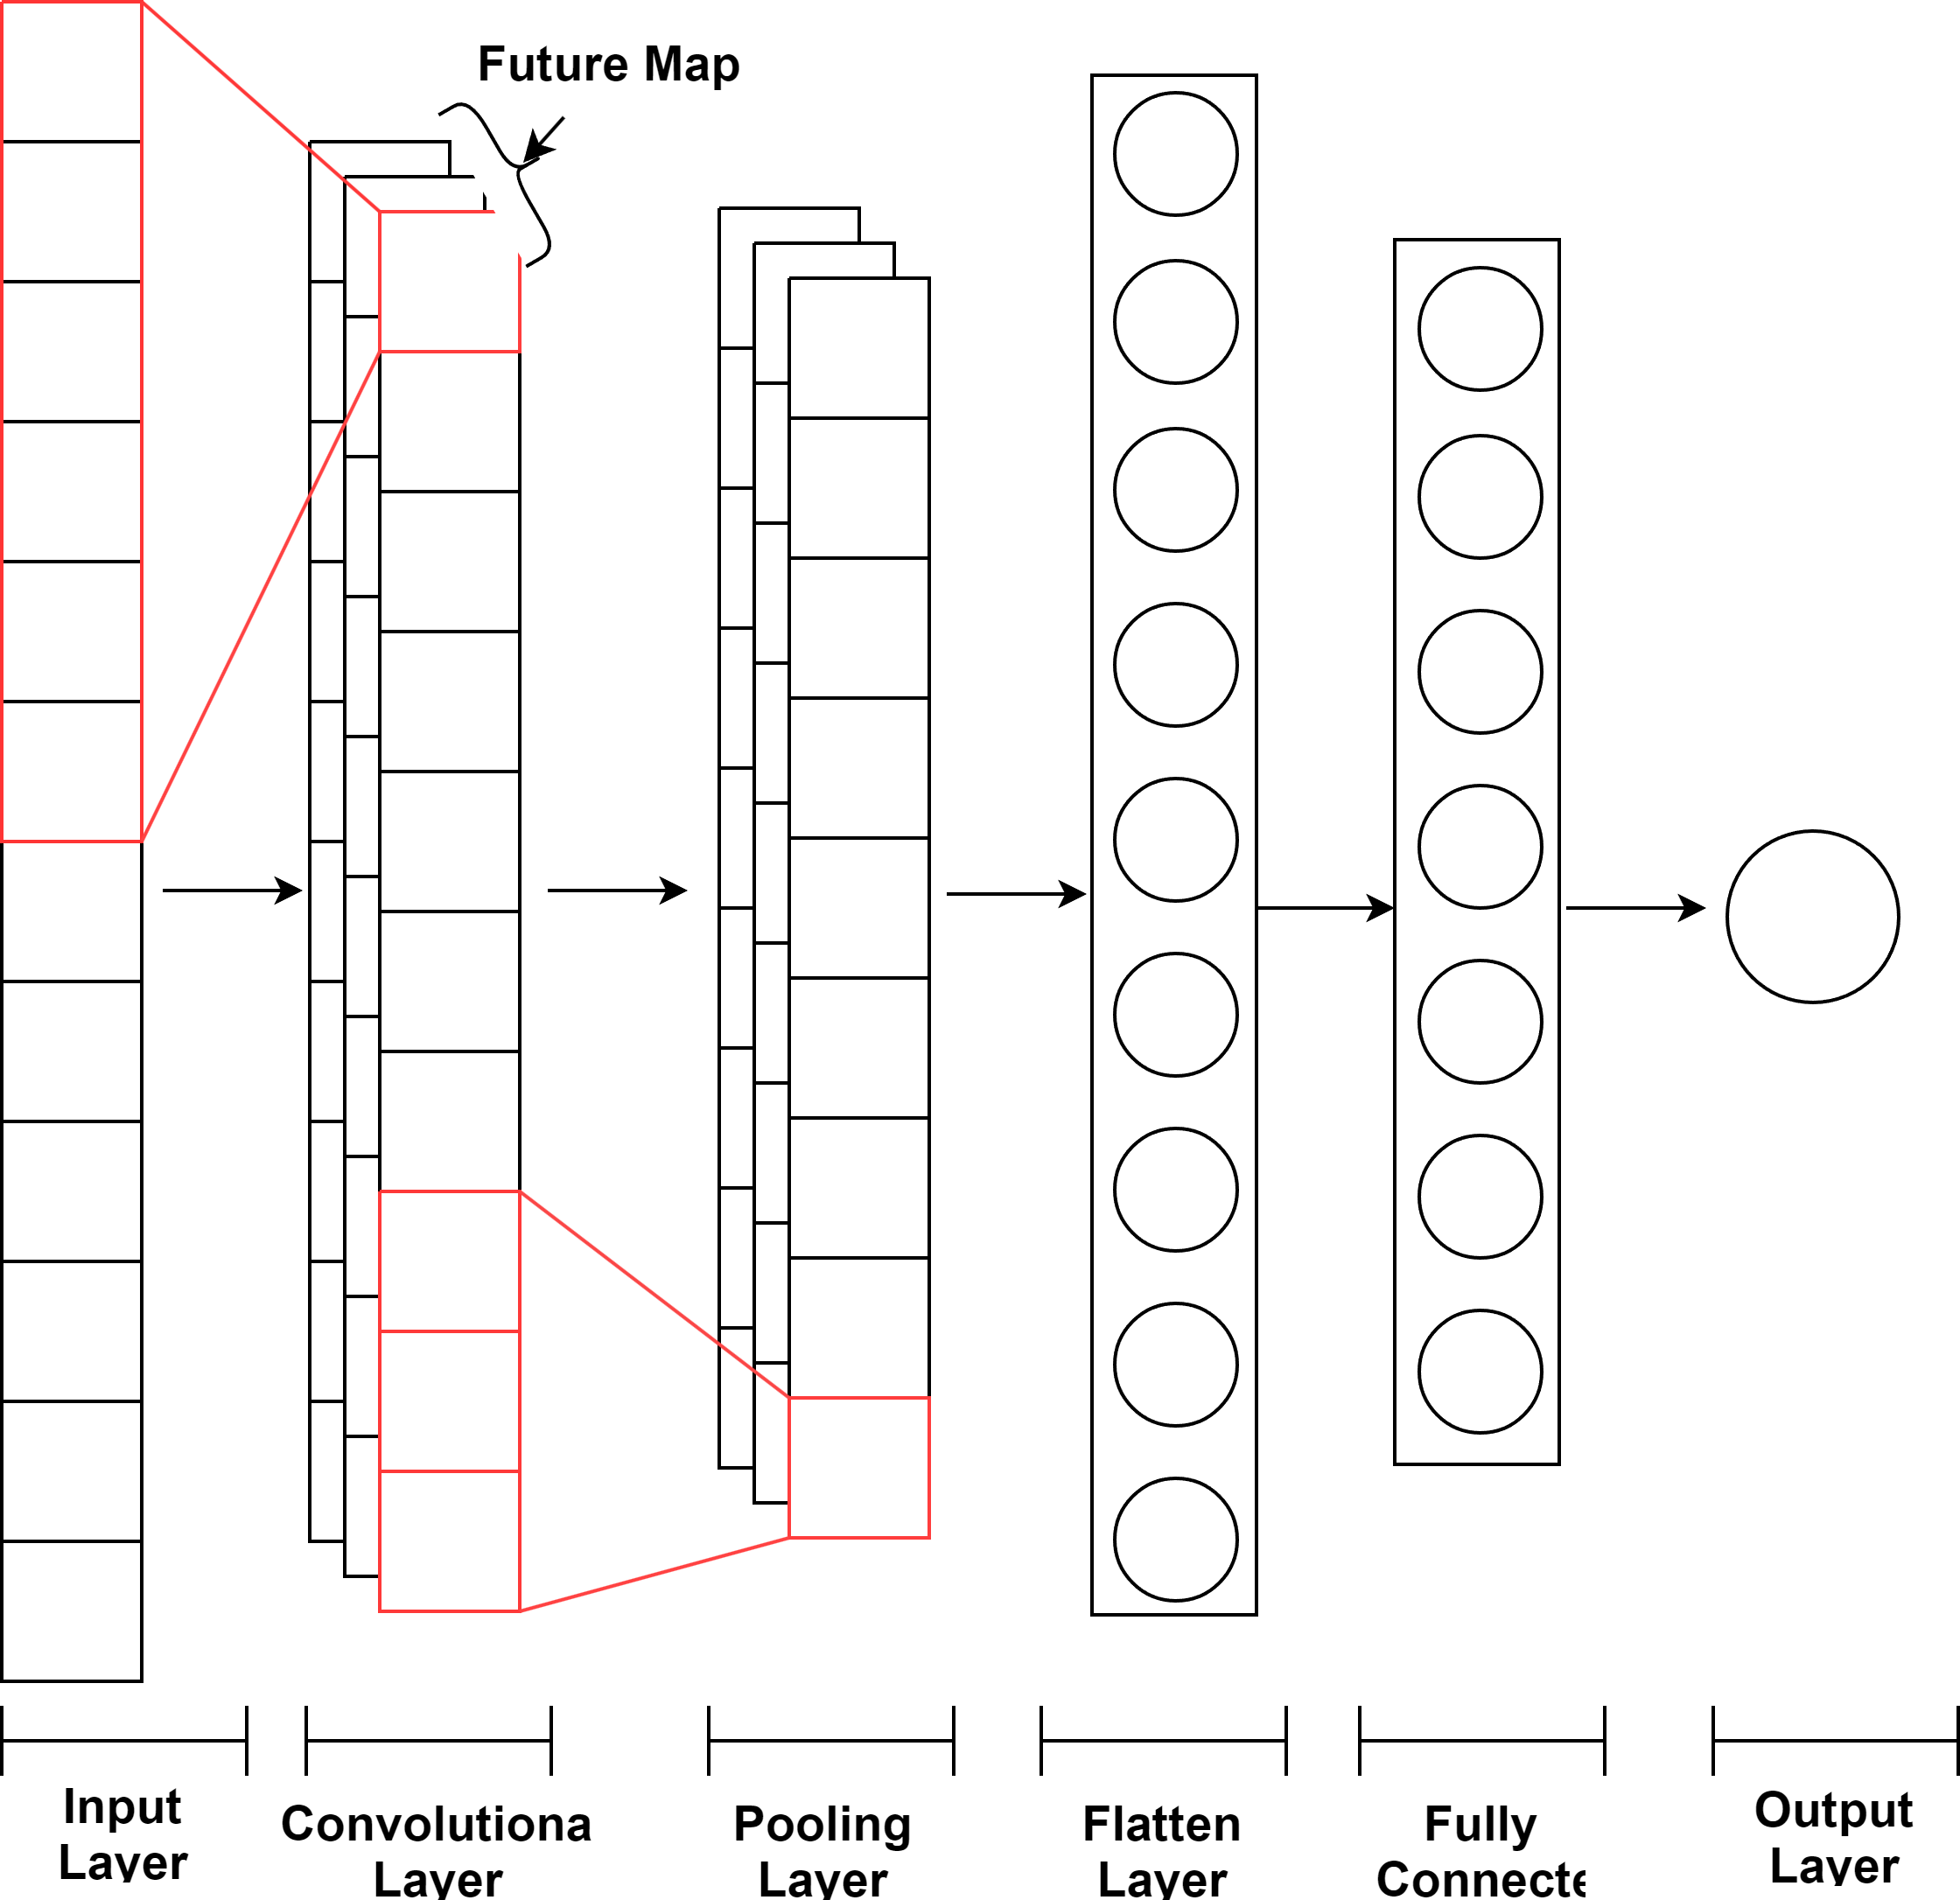
\includegraphics[scale=.8]{cnn}
    \caption{Traditional architecture of $1D-CNN$}\label{CNN}
\end{figure*}

1D CNN uses a set of learnable filters (or kernels) of length k to conduct the convolution operation. This operation involves computing the dot product between the filter and a k-length window sliding over the input sequence x with length L. Then a new sequence of feature maps is generated as an outcome.

\par Denoting the set of filters as $F$ and the output feature map at position $i$ as $h_i$,  we can express the output feature map $h$ as follows: 
\begin{equation}\label{equ: cnn}
        h_i = \sigma \left(\sum_{j=1}^{k}F_{j}.x_{i+j-1}+b \right)
\end{equation}
Where $F_j$ represents the $j^{th}$ filter in the set of filters $F$,  $x_{i+j-1}$ is the value of the input sequence $x$ at position $(i+j-1)$,  $\sigma$ is the activation function (such as ReLU or sigmoid),  and $b$ is the bias term.

\subsection{Gated Recurrent Unit (GRU)}
The GRU is a specialised recurrent neural network architecture designed for managing sequential data input  \cite{chung2014empirical}, and the unique proposal was put forth as a substitute for the well-liked LSTM network. These gating mechanisms selectively update the hidden state,  allowing GRU to capture dependencies in sequential data effectively. GRU has found use in an array of areas,  including speech recognition \cite{shewalkar2019performance, yuan2018auxiliary},  natural language processing \cite{cascianelli2018full, wang2020feature},  and picture recognition \cite{subramanian2022integrated},  due to its gating mechanisms and ability to handle sequential dependencies. Its capabilities make it a powerful tool for modelling and understanding sequential data,  providing valuable insights and improved performance in numerous tasks. GRU network based on gates and states are shown in \Cref{up Gru} to \Cref{hid gru}: \\
Update Gate :
\begin{equation} \label{up Gru}
  z_t= \sigma(W_{z}\cdot \left[ h_{t-1}, x_t \right]+b_z )
\end{equation}
Reset Gate : 
\begin{equation}\label{r gru}
 r_t=\sigma (W_{r}\cdot \left[ h_{t-1}, x_t \right]+b_r )
\end{equation}
Candidate activation :
\begin{equation} \label{can gru}
    \tilde{h_t}=tanh(W_h \cdot \left[ r_t \odot h_{t-1}, x_t \right]+b_h)
\end{equation}
Hidden State :  
\begin{equation} \label{hid gru}
  h_t=(1-z_t) \odot h_{t-1}+z_t \odot \tilde{h_t}
\end{equation}



where,  time step t,  the hidden state is represented by $ h_t $,  the input is represented by $ x_t $,  and the update and reset gates are
represented by $ x_t $ and $ r_t$ respectively. The refresh entryway directs the amount of the past covered state to keep for the present time step,  while the reset entryway controls the amount of the past covered state to overlook. The candidate activation $\tilde{h_t}$ represents new information that could be added to the hidden state. The sigmoid activation function $ \sigma $ and element-wise multiplication represented by $\odot$ are used.Weight matrices $ W_z $,  $ W_r $,  $ W_h $ and bias vectors $ b_z $,  $ b_r $,  $ b_h $ are also utilized. The GRU's update and reset gates allow it to learn when to update the hidden state and what information to forget,  making it particularly useful for modelling sequential data with long-range dependencies.
\subsection{Recurrent Neural Network (RNN)}
RNN is an ANN that utilises the outcome of the preceding measure to contribute to the present step. Forecasting the succeeding phrase in a statement is not a strong suit of RNNs because their Memory State,  also recognised as the hidden layer,  does not preserve any data about preceding words. It stores the previous input given to the network,  which goes a long way in ensuring accurate predictions. The RNN technique employs identical parameters for every input,  leading to it executing the same function on every hidden layer to obtain the results. Unlike other neural networks, it significantly reduces the complexity of parameters,  making it a popular choice among researchers and developers. The elegance of RNN rests in its capacity to recall prior inputs,  rendering it a valuable instrument in creating predictions that demand context. Ordinarily,  profound learning has been exhibited to be a game-changer in AI and ML,  and it will undoubtedly persist in being an essential instrument in the coming years.

Recurrent Neural Network (RNN) model are input \& output to hidden state can be written as \Cref{equ: ih rnn} \& \Cref{equ: h rnn} respectiveely: \\
Input to Hidden State:
  \begin{equation} \label{equ: ih rnn}
    h_t= \psi (W_{hx} \cdot x_t + W_{hh} \cdot h_{t-1} +b_h)
  \end{equation}
  Hidden State to Output: 
  \begin{equation} \label{equ: h rnn}
     y_t=W_{yh}\cdot h_t+b_y
  \end{equation}
where $h_t $ is the hidden state at time step $t$,  $x_t$ is input at $t$ step of time,  $y_t$ is output at t step of time,  $W_{hx} $ is a weight matrix that links the input to the concealed state,  $W_{hh}$ is the weighted matrix that connects the state that is hidden at time step $t-1$ with the hidden value step t,  $W_{yh}$ is a weighted matrix that links the state that is hidden to the output,  $b_h$ and $b_y$ are biassed terms for both the state that is hidden and the output and $\psi (\cdot)$ is a function of activation applied to the concealed state element by element.


\subsection{Long-Short-Term Memory (LSTM)}
LSTMs are a specialised type of RNN designed to handle sequential data. They excel at learning long-term dependencies,  making them suitable for language translation,  speech recognition,  and time series forecasting. Utilising the memory cell and three gates facilitates the capability of LSTMs to learn intricate patterns in data by selectively retaining and discarding information. Deep LSTM networks,  achieved by stacking LSTMs,  are beneficial for tasks like speech recognition \cite{soltau2016neural, jo2020approximate} and natural language processing \cite{wang2015learning, nammous2019natural}. Hochreiter and Schmidhuber  \cite{hochreiter1997long} developed LSTMs to overcome the long-term dependency issue in traditional RNNs. LSTMs are widely used in processing \cite{sahin2018nonuniformly},  prediction \cite{gers2000learning},  and classification \cite{zhou2015c, karim2017lstm} of temporal data,  and when combined with CNNs,  they efficiently analyse images \cite{li2019cnn, rajendran2020land, islam2020combined} and videos \cite{ullah2017action, li2020classifying, gao2017video, bin2018describing} by extracting spatial and temporal features. LSTMs are an effective instrument for analysing sequential data and can be incorporated with other neural network structures to accomplish more complex objectives.
The LSTM architecture-related gates and states are shown in \Cref{lstm i} to \Cref{lstm h}.\\
Input Gate : 
  \begin{equation} \label{lstm i}
     i_t=\sigma (W_{xi}\cdot x_t+W_{hi}\cdot h_{t-1}+b_i)
  \end{equation}
  Forget Gate : 
  \begin{equation}\label{lstm f}
    f_t= \sigma(W_{xf}\cdot x_t +W_{hf}\cdot h_{t-1}+b_f)
  \end{equation}
  Candidate Hidden State :
  \begin{equation}\label{lstm c}
       g_t=than(W_{xg}\cdot x_t+W_{hg}\cdot h_{t-1} +b_g)
  \end{equation}
  Cell State :
  \begin{equation}\label{lstm ce}
  C_t=f_t \odot C_{t-1}+i_t \odot g_t
  \end{equation}
  Output Gate : 
  \begin{equation}\label{lstm o}
    o_\sigma(W_{xo}\cdot x_t +W_{ho}\cdot h_{t-1}+b_o)
  \end{equation}
  Hidden State :
  \begin{equation} \label{lstm h}
      h_t=o_t \odot tanh(C_t)
  \end{equation}
whare,  $h_t$ at a time step,  is the concealed condition (also known as a hidden representation),  $x_t$  is the time step input,  $C_t$  is the condition of the cell at time step $t$,  serving as the LSTM's long-term memory,  $\sigma$ Its sigmoid activation function,  The tangent hyperbolic activation function is denoted by tanh,  $\odot$ represents element-by-element multiplication,  $W_{xi}$,  $W_{hi}$,  $W_{xj}$,  $W_{hf}$,  $W_{xg}$,  $W_{hg}$,  $W_{xo}$,  $W_{ho}$ are the matrices of that will be taught throughout training and $b_i$,  $b_f$,  $b_g$,  $b_o$ are slanted terms.


\subsection{Bi-directional Long Short Term Memory (BiLSTM)}
BiLSTM is a type of human stupidity designed to process sequential data in neither forward nor backward directions. The plan uses dual LSTM layers for forward and backward processing concurrently,  enabling it to grasp the context from previous and upcoming time steps. Therefore,  the network cannot identify any relationships in either direction,  making it a disadvantage for speech recognition and language translation tasks. By providing a broader perspective of the input sequence,  BiLSTMs can improve the performance in tasks requiring contextual understanding. These forms are remarkable for long-term dependencies and are commonly utilised in profound learning projects.

\begin{figure*}[h!]
  \centering
  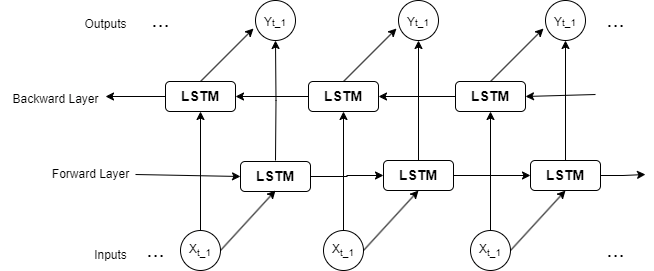
\includegraphics[scale=0.8]{Bilstm}
  \caption{Architecture of BiLSTM \cite{article}} \label{Bilstm}
\end{figure*}



BiLSTM network architecture gates and states are shown below from \Cref{bi i} to \Cref{bi h}.\\
\begin{itemize}
  \item  Forward LSTM: \\
  Input Gate : 
    \begin{equation} \label{bi i}
    i_t^f = \sigma(W_{xi}^f \cdot x_t + W_{hi}^f \cdot h_{t-1}^f + W_{ci}^f \cdot c_{t-1}^f + b_i^f)
    \end{equation}
    Forget Gate : 
    \begin{equation}
      f_t^f = \sigma(W_{xf}^f \cdot x_t + W_{hf}^f \cdot h_{t-1}^f + W_{cf}^f \cdot c_{t-1}^f + b_f^f) 
    \end{equation}
    Candidate Hidden State :
    \begin{equation}
        g_t^f = \text{tanh}(W_{xg}^f \cdot x_t + W_{hg}^f \cdot h_{t-1}^f + b_g^f)
    \end{equation}
    Cell State : 
    \begin{equation}
      c_t^f = f_t^f \odot c_{t-1}^f + i_t^f \odot g_t^f
    \end{equation}
    Output Gate : 
    \begin{equation}
   o_t^f = \sigma(W_{xo}^f \cdot x_t + W_{ho}^f \cdot h_{t-1}^f + W_{co}^f \cdot c_t^f + b_o^f)
    \end{equation}
    Hidden State : 
    \begin{equation} \label{bi h}
    h_t^f = o_t^f \odot \text{tanh}(c_t^f) 
    \end{equation}

  \item Backward LSTM: 
  The formulas for the rear LSTM are similar to those of the forward LSTM but with different weights and biases. The superscript "b" is used to denote the backward direction (e.g.,  \(W_{xi}^b\) is the weight matrix for the input gate in the backward LSTM). The BiLSTM combines the hidden forward and backwards states to form the final output. The output \(y_t\) at time step \(t\) is typically computed using a combination of both forward and backwards hidden states. The approach for combining the two directions (e.g.,  concatenation,  addition,  etc.) depends on the specific task and model architecture.
\end{itemize}

\section{ Performance Measures}
\subsection{Root Mean Square Error (RMSE) }
The RMSE is hardly ever utilised as a standard for assessing the precision of a regression model. The computation of the root mean square of discrepancies between projected and factual figures can facilitate identifying the divergence between them while keeping the units of measurement consistent with the data. This provides valuable insight into the model's effectiveness. A lower RMSE digit suggests superior model performance,  while an increased RMSE value indicates substandard model performance. The RMSE \Cref{rmsee} uses metrics for regression models by effectively evaluating the model's accuracy,  as it quantifies the discrepancy between projected and actual values in the same unit as the data. By analysing the RMSE score,  experts can evaluate the model's efficacy and implement necessary tweaks to enhance its precision. As a final point,  the RMSE is a crucial statistic for evaluating the accuracy of regression models,  and its usage is essential in industries that heavily depend on data science,  finance,  and engineering.

\begin{equation} \label{rmsee}
  RMSE=\sqrt{\frac{\sum_{i=1}^{n}(y_{i}-\hat{y_{i}})^2}{n}}
\end{equation}
where $n$ represents the number of times that the summation iteration occurs,  \begin{math} y_{i} \end{math} denotes the actual value,  and \begin{math}\hat{y_{i}}\end{math} represents the forecast value.

\subsubsection{ Mean Absolute Percentage Error (MAPE)}
  A popular metric for judging the efficiency of regression models is MAPE. It measures the percentage of variance between predicted and actual results and averages these discrepancies. MAPE can be computed by finding the average of the absolute percentage errors between the expected and actual values,  such as \Cref{mapee}.
\begin{equation} \label{mapee}
  MAPE=\frac{1}{n}\sum_{i=1}^{n} \left | \frac{y_{i}-\hat{y_{i}}}{y_{i}} \right |
\end{equation}
where $n$ represents the number of times that the summation iteration occurs,  \begin{math} y_{i} \end{math} denotes the Actual value,  and \begin{math}\hat{y_{i}}\end{math} represents the forecast value.

MAPE determines the average percentage discrepancy between the projected and observed values. In business and finance,  it is a common practice to assess the precision of forecasts or predictions using this technique. Industries utilise MAPE to compute the mean percentage deviation between anticipated and actual values,  where a lower value suggests better model performance and a higher value suggests poorer performance. However,  MAPE can cause division by zero errors or huge percentage errors when the actual numbers are close to zero.




%% Chapter Template

\chapter{Methodology} % Main chapter title

\label{c4} % Change X to a consecutive number; for referencing this chapter elsewhere, use \ref{ChapterX}


 
% \section{Methodology}
This section describes the methodology for tracking accurate temperature prediction using DL techniques on time series data originating from Delhi. The foundation of our study rests on the comprehensive collection and preprocessing of temperature data. We sourced our dataset from reputable weather stations in Delhi from the NASA website, spanning a specific period critical for climate analysis. We conducted rigorous cleaning procedures to ensure data integrity, handle missing values, detect and address outliers, and remove duplicates. Additionally, we performed feature engineering to extract relevant temperature-related features, enhancing the granularity of our Dataset for DL model input.

The exploration of the data's underlying characteristics was undertaken through Exploratory Data Analysis (EDA). Visualization tools, such as line plots and histograms, facilitated the identification of critical temporal patterns and anomalies within the temperature time series. Statistically, we employed various analytical methods during EDA to unveil underlying trends and seasonality.

We selected the LSTM, Bi-LSTM, GRU and RNN DL architecture for the heart of our temperature prediction. Bi-LSTM networks are well-suited for modelling sequential data and capturing long-term dependencies, making them a natural choice for time series forecasting. To optimize model performance, we meticulously tuned hyperparameters, including network depth, hidden unit configurations, activation functions, and dropout rates.



\begin{figure}[ht!]
\centering
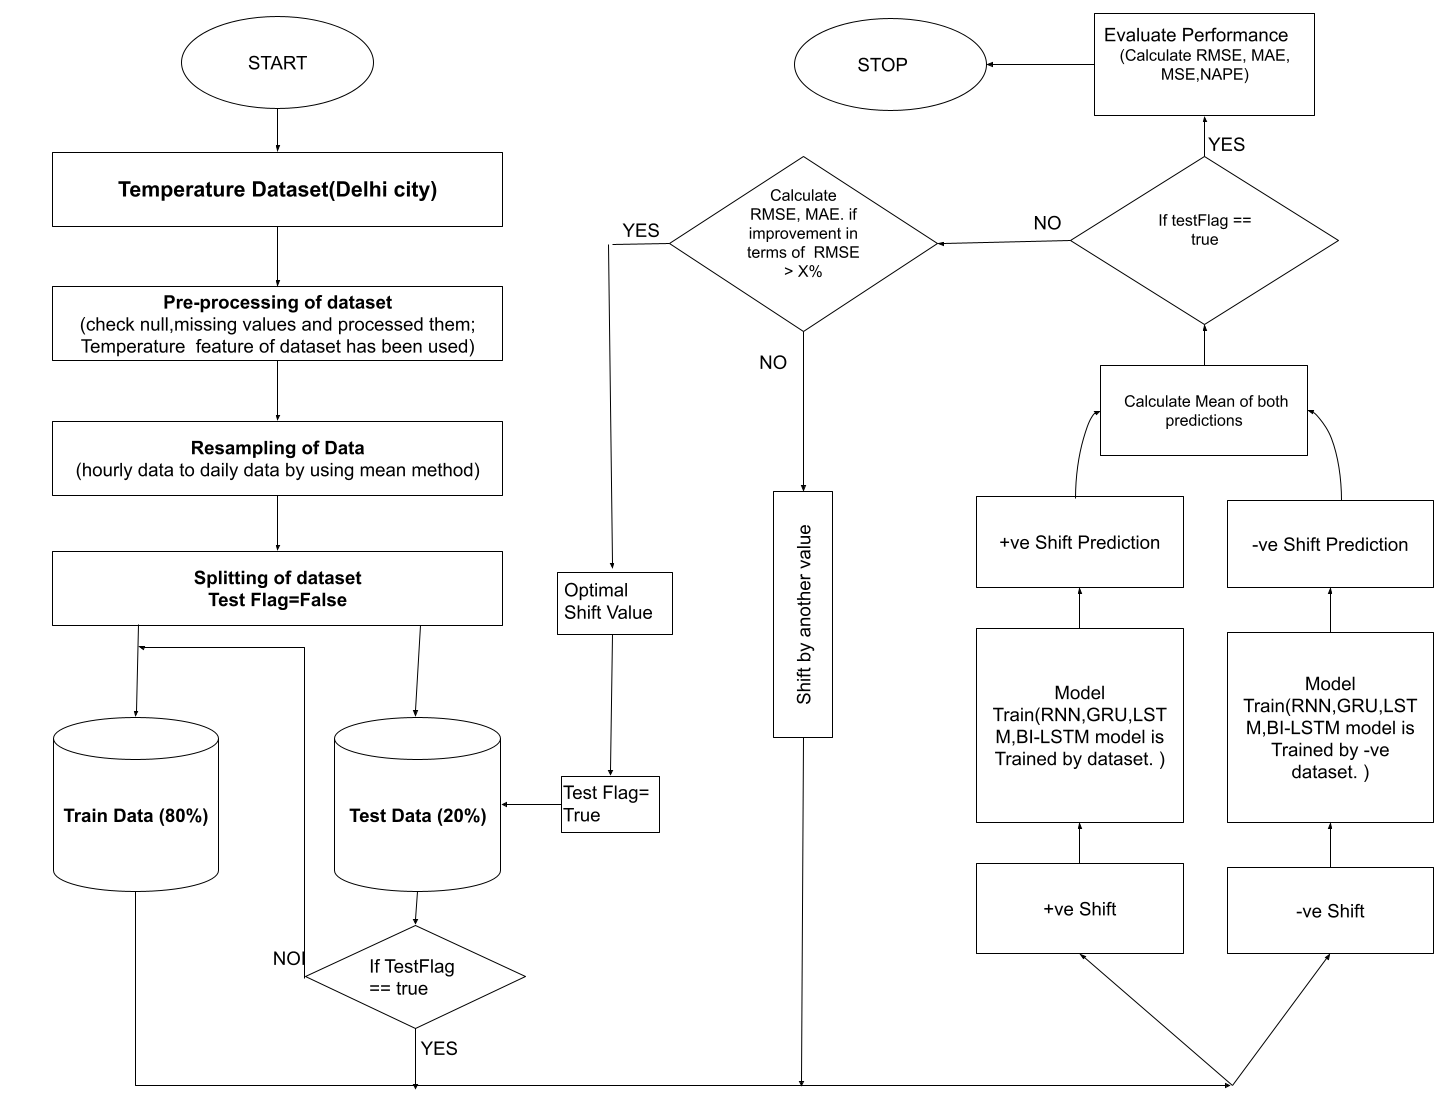
\includegraphics[width=1\textwidth, height=0.9\linewidth]{FlowchartOfjournal.png}
\caption{Framework of the proposed work MBiS-DT + DL models}
\label{fig:Flowchart Of Proposed Work}
\end{figure}
\section{Data collection and preprocessing}
\subsection{Raw dataset collection}
The dataset used in this study is publicly accessible on NASA's website . The dataset contains 195101 rows in CSV format of temperature and dew point of New Delhi from 02/01/2001 to 06/04/2023 on an hourly frequency. The T2M are distinct kinds of atmospheric conditions. These conditions define the atmosphere's temperature for each record in the dataset D, shown in eqn. (\ref{eqn:d}).

\begin{equation}
\label{eqn:d}
D=\left \{ x_i, y_i \right \}_{i=1}^{k}
\end{equation}

where, D is denoted as dataset, \(x_i\) is a temperature data of hours interval, and \(y_i\) its corresponding time. k denotes the number of samples in the dataset, $\forall y_i \in y $.

\subsection{Data preprocessing}
This technique phase consists of four phases. First, dataset D has been resized into a new dimension daily. The function representing the dimension is omega. As shown in eqn.- (\ref{eqn:c}), we also organized the data by date and time and examined the dataset's non-linearity. Furthermore, temperature(T2M) values between 2001 and 2023 have been chosen from the resized dataset. Each date from January 2, 2001, to April 6, 2023, is placed in the dependent variable column, and each item in that column of time series data for 22 years (2001-2023) having temperature (T2M) as an independent variable column has been added.

\begin{equation}
\label{eqn:c}
D_{new}=\omega \left ( D, p \times q \right )
\end{equation}

where, \(D_{new}\) is the preprocessed the dataset D. Here, p x q are the new dimension of the dataset.
\subsection{Exploratory data analysis(EDA)}

% \begin{table*}[h!]
% \caption{statistical summarization of Data set}
% \label{tab: statistical_data_explore }
% \begin{tabular}{ll}
% \hline parameters & Values \\ \hline
% count & 195101 \\
% mean & 25.10 \\
% std & 21.73 \\
% min & -999 \\
% 25\% & 18.70 \\
% 50\% & 26.46 \\
% 75\% & 31.98 \\
% max & 48.79 \\ \hline
% \end{tabular}
% \end{table*}
This section explains statistical details about our Delhi temperature dataset. It provides insights into the dataset's size, central tendency, variability, distribution, and range. These statistics serve as a foundational resource for analyzing and interpreting temperature trends in Delhi, supporting various climate-related studies, weather forecasts, and informed decision-making processes. The \textbf{"count"} value 8,128 indicates the dataset's size, revealing that it bound a substantial number of temperature observations or data points. This size underscores the dataset's richness and the depth of information available for analysis, offering a robust foundation for temperature-related insights. The \textbf{"mean"} temperature of 25.49 degrees serves as the arithmetic average of the dataset. It suggests that, on average, the recorded temperatures in Delhi hover around 25.49 degrees. This central tendency measure offers a crucial reference point, representing the typical temperature value within the dataset. The \textbf{"standard deviation"} (std) of 7.77 quantifies the degree of temperature variation or dispersion in the data. A higher standard deviation indicates more significant variability in the recorded temperatures. In this case, the standard deviation of 7.77 implies that temperature readings in Delhi can exhibit substantial fluctuations around the Mean, signifying the presence of diverse temperature patterns.

The \textbf{"min"} value of 6.95 is the most minor observed temperature in the dataset. However, this value appears unusual and may require further investigation. Some previous Values, like -999, often signify missing data or anomalies that warrant scrutiny to ensure data quality and integrity, so it is handled by taking the Mean of the successor and predecessor value of the time-series dataset. The \textbf{"max"} value of 41.81 denotes the highest temperature recorded in the dataset, offering a glimpse into the upper limit of temperature extremes experienced in Delhi. The \textbf{quartile} values—25\% (first quartile), 50\% (median), and 75\% (third quartile)—offer valuable insights into the distribution of temperatures in Delhi. The first quartile at 18.73 indicates that 25\% of temperature readings fall below this level, while the third quartile at 31.48 signifies that 75\% of the temperatures are below this threshold. The median value of 26.85, also the second quartile, represents the middle point of the dataset when arranged in ascending order. Notably, the median is a robust measure of central tendency unaffected by extreme outliers. These quartile values provide context for understanding the spread and distribution of temperature data in Delhi.



\begin{figure}[ht!]
\centering
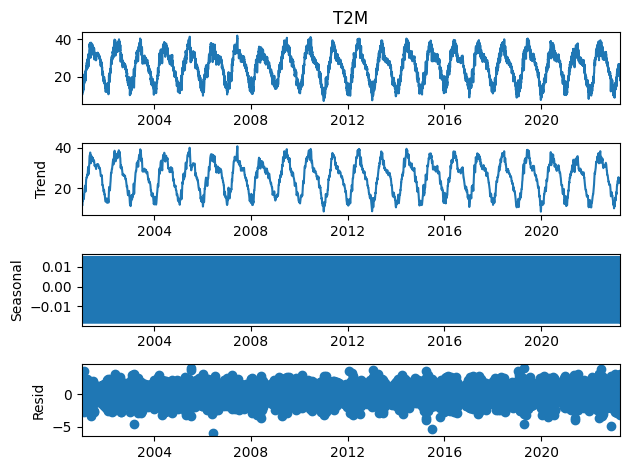
\includegraphics[width=1\textwidth, height=0.75\linewidth]{Graphycal_EDA.png}
\caption{The decomposition of data as a trend, seasonal and residual of Jan. 2001 to Sept. 2001. }
\label{fig:graphycalEDA}
\end{figure}
In our dataset, a good trend is visualized. A trend represents a substantial and meaningful long-term pattern in temperature variations. This pattern provides the fundamental direction in which the 2-meter air temperature changes over an extended period. In climate science, recognizing such trends is vital for understanding the dynamics of temperature variations over time, whether the moderate warming associated with climate change or the multi-year temperature cycles linked to climate phenomena like Delhi. Accurately identifying and modelling these trends is pivotal for climate scientists and meteorologists, as it enables them to make informed projections about future temperature changes, prepare for potential impacts, and implement mitigation strategies.
In the context of our temperature dataset, \textbf{"seasonality"} represents the regular and cyclical fluctuations in temperature that occur at consistent intervals throughout the year. These fluctuations often align with the changing seasons, resulting in patterns like warmer temperatures during summer and colder temperatures during winter. Seasonality in T2M data can be attributed to various factors, including the tilt of the Earth's axis, which leads to variations in sunlight exposure throughout the year. Identifying seasonality in temperature data is critical for climate scientists and ecologists, as it aids in understanding the impact of changing seasons on ecosystems \cite{liu2021modeling}, agriculture \cite{murugesan2021deep}, and human activities. This knowledge is crucial for crop planning\cite{sehgal2017crop}, energy demand forecasting\cite{choi2020power}, and environmental conservation efforts\cite{lee2017using}.

Residuals in our temperature dataset refer to unexplained fluctuations or variations after accounting for the identified trends and seasonality. These residuals represent the difference between the observed 2-meter air temperatures and the values predicted by a model incorporating long-term trends and seasonal patterns. In climate research, analyzing residuals is vital for assessing the accuracy of climate models and identifying any irregular or unanticipated temperature fluctuations. Residuals should exhibit no systematic patterns; if they do, it suggests that the model may need refinement to capture the underlying dynamics of temperature changes better. Effective handling of residuals is essential for producing reliable temperature predictions, which, in turn, inform climate policy\cite{gilik2022air}, weather forecasts\cite{shin2021short}, and resilience planning\cite{ghaith2022synchronization} in the face of temperature-related challenges \cite{lee2020forecasting}.
% \section{Train, and Test Splitting of Dataset}



% \par {\textbf{Step 4}: Applying Deep Learning Models:}\\ the model \(\emptyset\left(D_{Tr}\ ,\ D_{Te}\right)\) has been applied. The forecasting for the test sample has been obtained in the model's training and test part. Prediction is obtained:\(\left\{P_i^\emptyset\right\}_i^m\), where m is number of test sample %\cite{hrithik2022classification}.

% \par {\textbf{Step 5}: Root Mean Squared Error:}\\ RMSE is calculated by eqn. \ref{eqn:e}.



% Where N is total no of test Sample, \(\hat{y_{i}}\) is a predicted data of model, and \(y_{i}\) is the actual test deta.\\
% \par {\textbf{Step 6}: Proposed Technique:} \\
\section{Proposed Multi-Bidirectional Shifting based Data Transformation(MBiS-DT) with DL Model}
\begin{figure}[ht!]
\centering
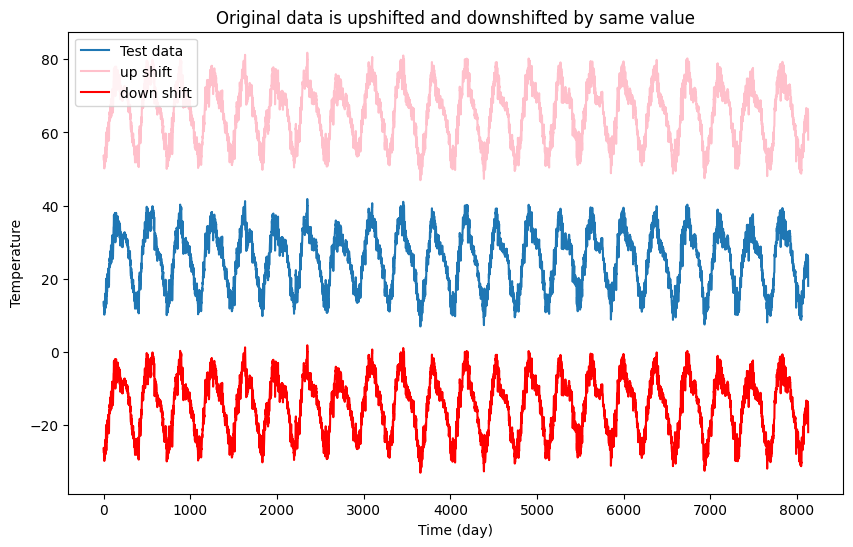
\includegraphics[scale = 0.4]{shifted_dataset.png}
\caption{Pictorial representation of Multi-Bidirectional shifting based Data Transformation(MBiS-DT) for multiple DL learning for the ensemble of models.}
\label{fig:shifted_dataset}
\end{figure}
The preprocessed dataset has been divided into two parts: training \((T_{train})\) (80\%) and testing \((T_{test})\) (20\%). The dataset is mutually exclusive in eqn. (\ref{eqn:a}) and exhaustive in eqn. (\ref{eqn:b}).

\begin{equation}
\label{eqn:a}
D_{T}=D_{Tr}\cup D_{Te}
\end{equation}

\begin{equation}
\label{eqn:b}
\left \{ D_{Tr} \cap D_{Te} \right \}=\varnothing
\end{equation}

For the data points $x_i$ in the training dataset $D_{Tr}$, two series can be created as in eqn. (\ref{eqn:01}):
\begin{equation}
\begin{aligned}
\label{eqn:01}
\{x_i^{\prime}=x_i+s\}_{i=1}^n \\
\{x_i^{\prime\prime}=x_i-s\}_{i=1}^n \; \forall x_i \in D_{Tr}
\end{aligned}
\end{equation}
where $s \in Z$ and $x_i^{\prime}$ and $x_{i}^{\prime\prime}$ depicts the positive and negative series obtained by shifting the series with positive and negative values of the step length $s$ of the shift. The series has been prepared for $n$ number of iterations.
Predictions for both the positive $x_i^{\prime}$ and negative $x_i^{\prime\prime}$ series has been obtained as $\hat{y}_i^{\prime}$ and $ \hat{y}_i^{\prime\prime}$ respectively.
The predictions are combined to form a final set of predictions using eqn. (\ref{eqn:02}), which is utilized to compare with the actual values of training dataset $D_{Tr}$.
\begin{equation}
\label{eqn:02}
\hat{y}_{final}=\frac{y_i^{\prime}+y_i^{\prime\prime}}{2}
\end{equation}
where $\hat{y}_{final}$ represents the final prediction. The above procedure is repeated for $n$-number of iterations, and an optimal value of $s$ is obtained for which the RMSE is best out of $n$-number of iterations.
Then, the model is trained for the actual training data $D_{Tr}$, and predictions are obtained for the test data $D_{Te}$, which is $D_{Te}^{\prime}$. Further, two positive and negative series are obtained from test prediction $D_{Te}^{\prime}$ as reflected in eqn. (\ref{eqn:03}).
\begin{equation}
\begin{aligned}
\label{eqn:03}
\{x_j^{\prime}=x_j+s\} \\
\{x_j^{\prime\prime}=x_j-s\} \; \forall x_j \in D_{Te}^{\prime}
\end{aligned}
\end{equation}
where $s$ is the step length obtained earlier and $x_j^{\prime}$ and $x_{j}^{\prime\prime}$ depicts the positive and negative series obtained by shifting the series with positive and negative values of the step length $s$ of the test predictions $ D_{Te}^{\prime}$.
Predictions for both the positive $x_j^{\prime}$ and negative $x_j^{\prime\prime}$ series has been obtained as $ \hat{y}_j^{\prime}$ and $ \hat{y}_j^{\prime\prime}$ respectively.

The predictions are combined to form a final set of predictions using eqn. (\ref{eqn:04}), which is utilized for the comparison with the actual values of training dataset $D_{Te}$
\begin{equation}
\label{eqn:04}
\hat{y}_{final}^{\prime}=\frac{\hat{y}_j^{\prime}+\hat{y}_j^{\prime\prime}}{2}
\end{equation}
where $\hat{y}_{final}^{\prime}$ represents the final prediction.




% \begin{figure}[ht!]
% %\centering
% \subfloat[Test data vs Proposed MBiS-DT GRU] {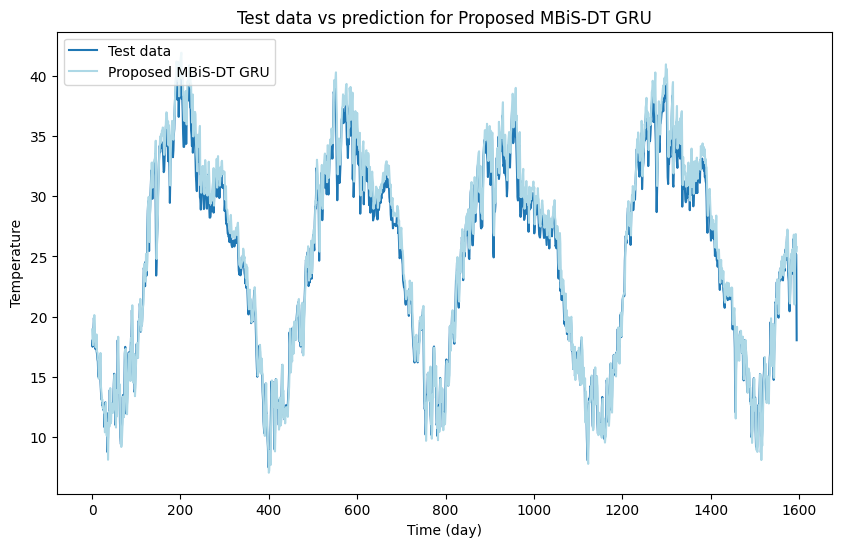
\includegraphics[scale=0.3]{testData_vs_proposed_GRU.png}\label{fig:BarPlot_TestDataVSMBiS-DT_GRU}}
% \hfill
% \subfloat[Test data vs Proposed MBiS-DT RNN]{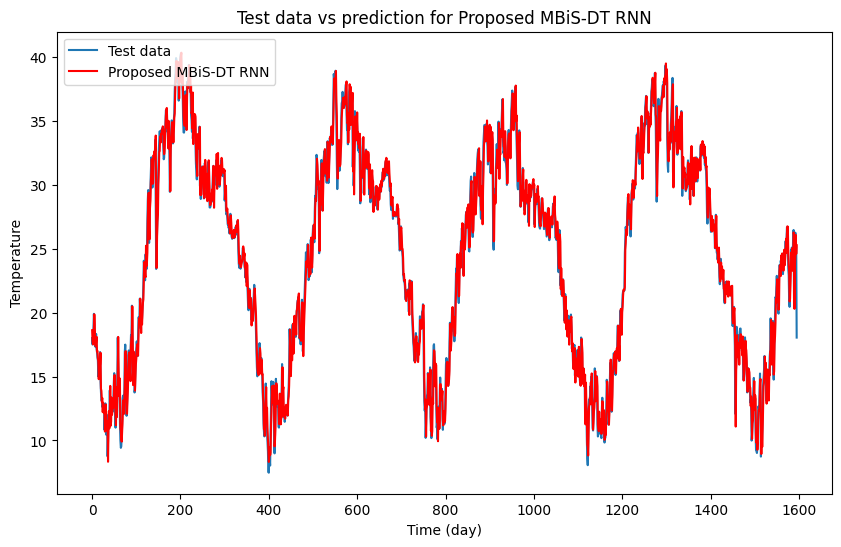
\includegraphics[scale=0.3]{testData_vs_proposed_RNN.png}\label{fig:BarPlot_TestDataVSMBiS-DT_RNN}}\\
% \subfloat[Test data vs Proposed MBiS-DT BI-LSTM]{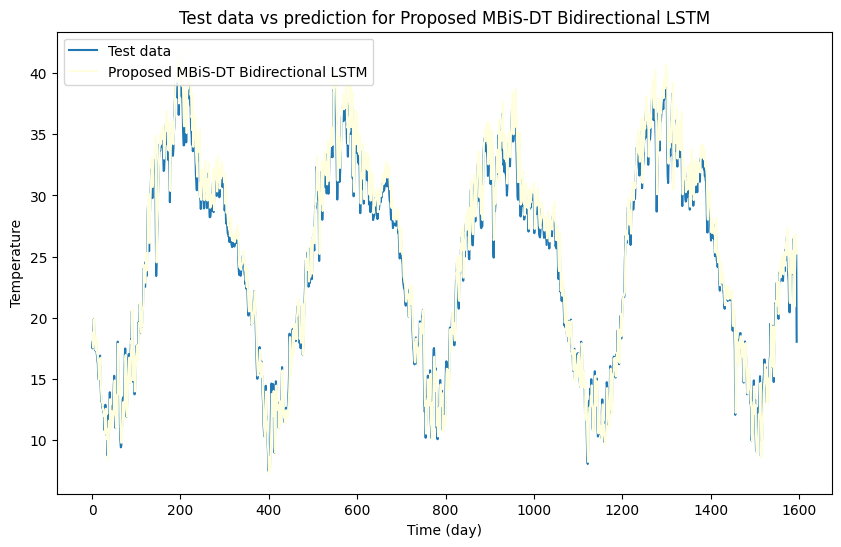
\includegraphics[scale=0.3]{testData_vs_proposed_BI-lstm.png}\label{fig:BarPlot_TestDataVSMBiS-DT_BILSTM}}
% \hfill
% \subfloat[Test data vs Proposed MBiS-DT LSTM]{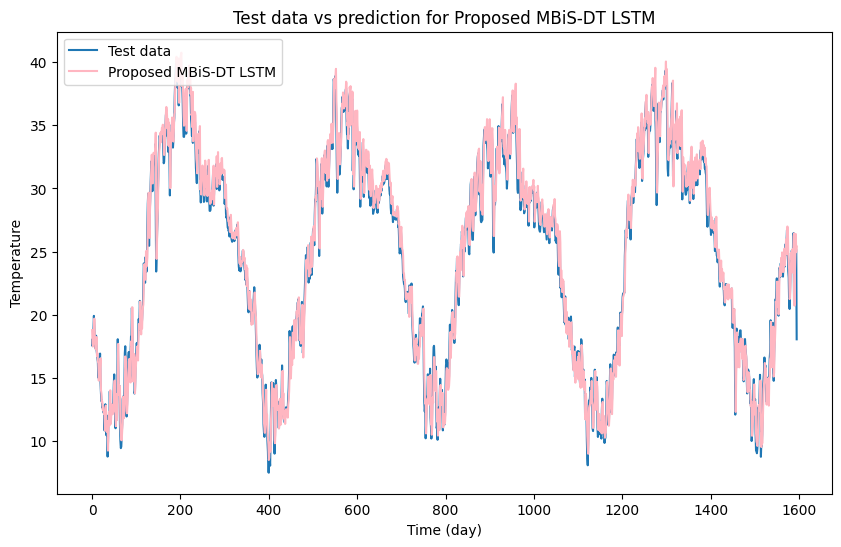
\includegraphics[scale=0.3]{testData_vs_proposed_LSTM.png}\label{fig:BarPlot_TestDataVSMBiS-DT_LSTM}}
% \caption{Prediction plot of original test data(subset) corresponding to traditional DL models and proposed MBiS-DT + DL's models.}
% \label{fig:Line plot of vs proposed MBiS-DT models}
% \end{figure}



% \begin{figure}[ht!]
% \centering
% 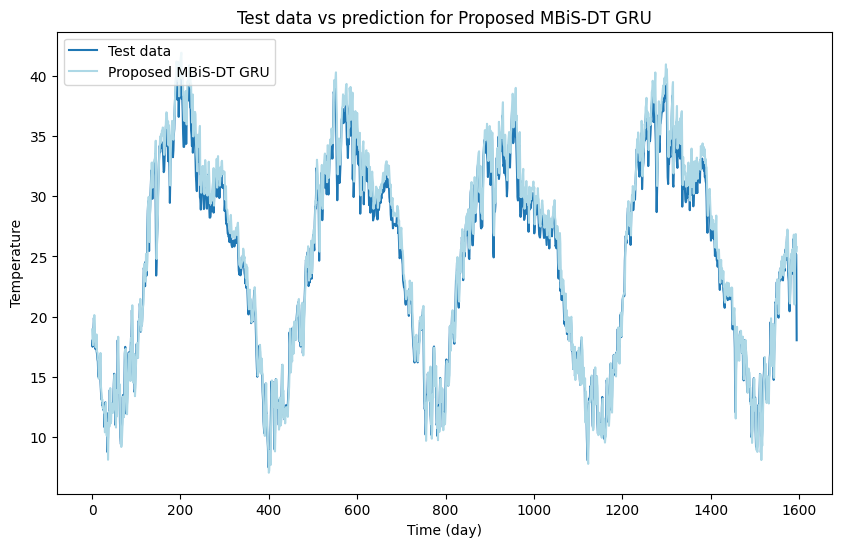
\includegraphics[width=1\textwidth, height=0.9\linewidth]{testData_vs_proposed_GRU.png}
% \caption{Test data vs Proposed MBiS-DT GRU}
% \label{fig:BarPlot_TestDataVSMBiS-DT_GRU}
% \end{figure}
% \begin{figure}[ht!]
% \centering
% 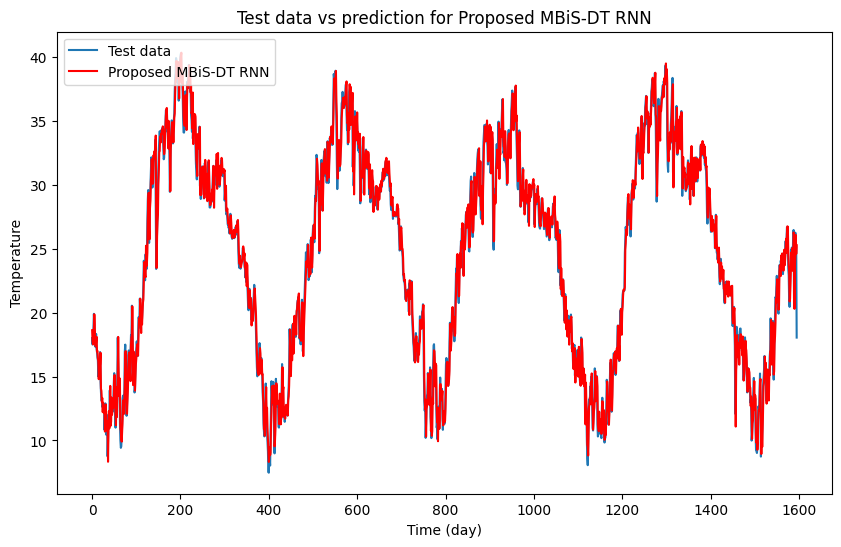
\includegraphics[width=1\textwidth, height=0.9\linewidth]{testData_vs_proposed_RNN.png}
% \caption{Test data vs Proposed MBiS-DT RNN}
% \label{fig:BarPlot_TestDataVSMBiS-DT_RNN}
% \end{figure}
% \begin{figure}[ht!]
% \centering
% 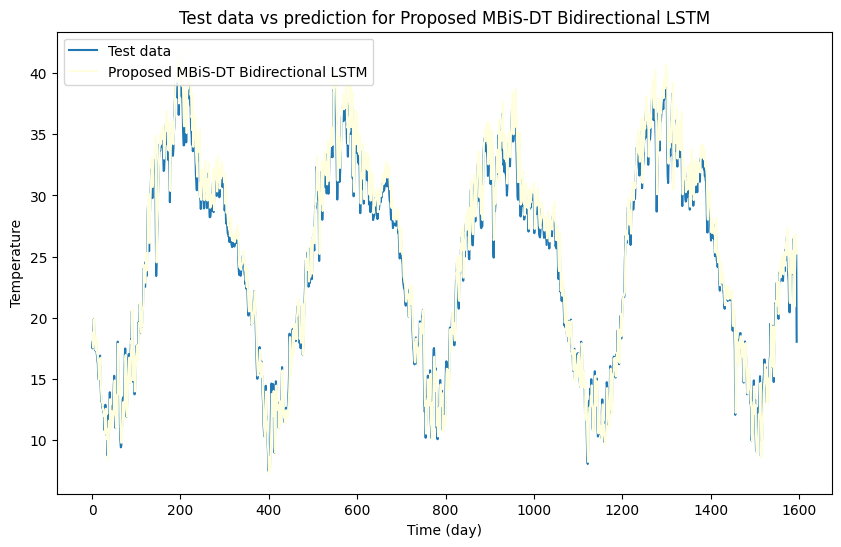
\includegraphics[width=1\textwidth, height=0.9\linewidth]{testData_vs_proposed_BI-lstm.png}
% \caption{Test data vs Proposed MBiS-DT BI-LSTM}
% \label{fig:BarPlot_TestDataVSMBiS-DT_BILSTM}
% \end{figure}
% \begin{figure}[ht!]
% \centering
% 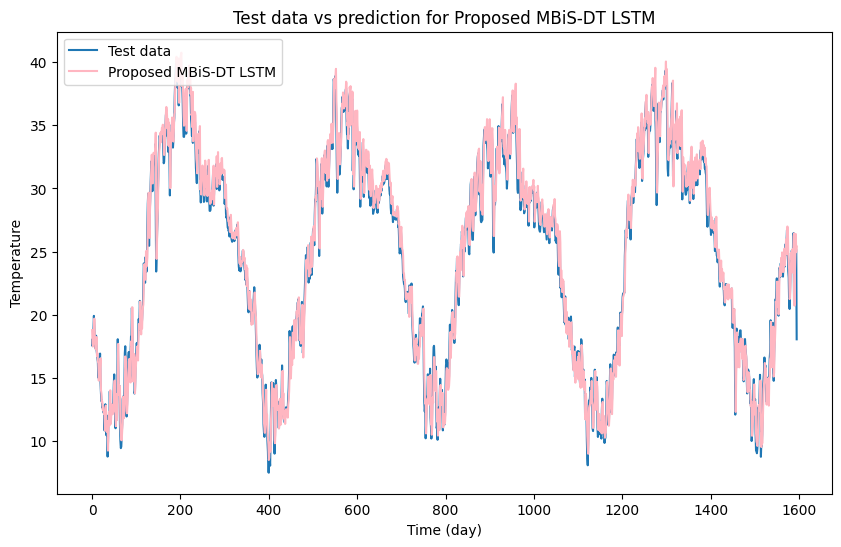
\includegraphics[width=1\textwidth, height=0.9\linewidth]{testData_vs_proposed_LSTM.png}
% \caption{Test data vs Proposed MBiS-DT LSTM}
% \label{fig:BarPlot_TestDataVSMBiS-DT_LSTM}
% \end{figure}



% \begin{figure}[ht!]
% %\centering
% \subfloat[Test data vs Proposed MBiS-DT GRU] {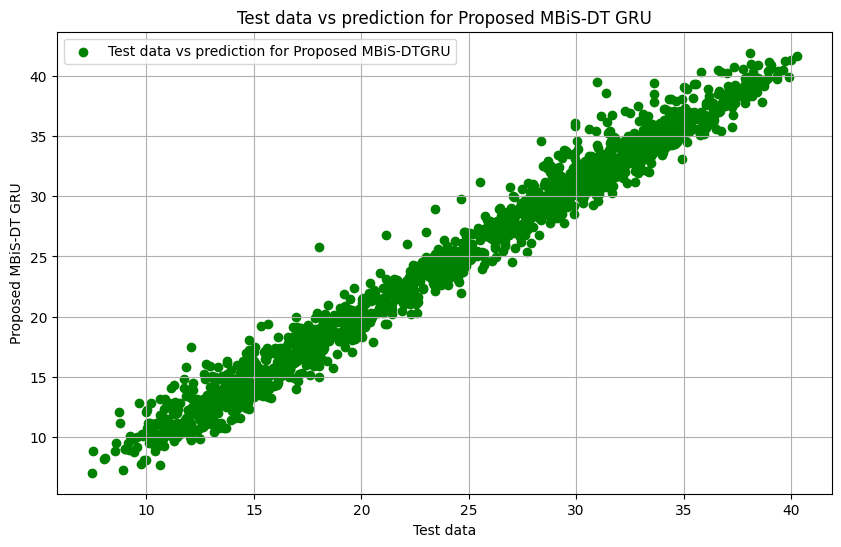
\includegraphics[scale=0.3]{scatter_gru.png}\label{fig:ScatterPlot_TestDataVSMBiS-DT_GRU}}
% \hfill
% \subfloat[Test data vs Proposed MBiS-DT RNN]{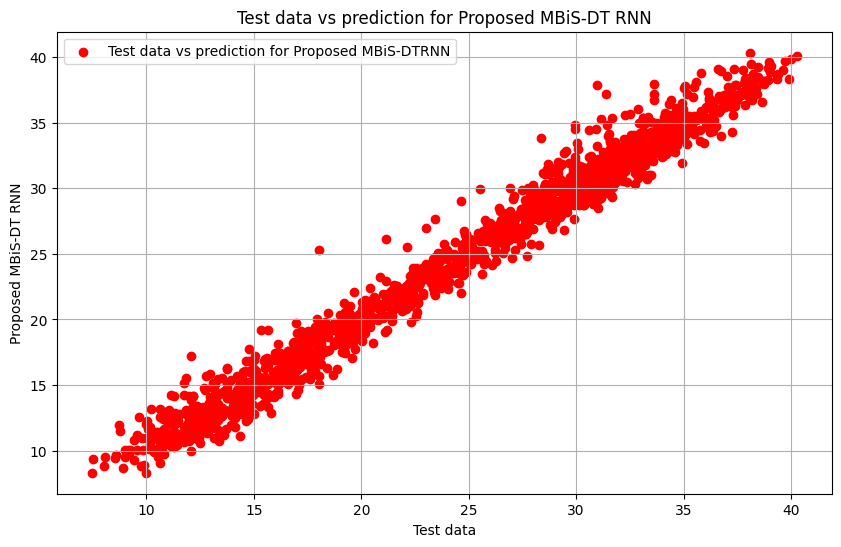
\includegraphics[scale=0.3]{scatter_rnn.png}\label{fig:ScatterPlot_TestDataVSMBiS-DT_RNN}}\\
% \subfloat[Test data vs Proposed MBiS-DT BI-LSTM]{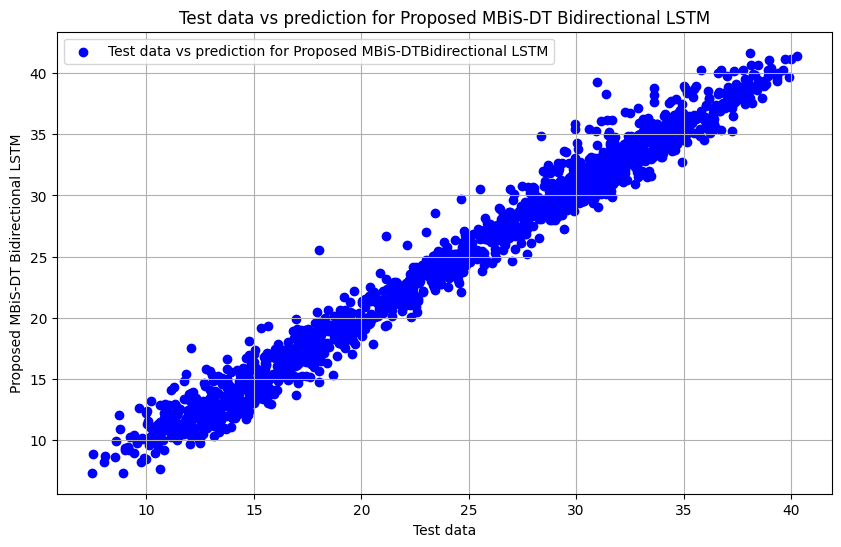
\includegraphics[scale=0.3]{scatter_bilstm.png}\label{fig:ScatterPlot_TestDataVSMBiS-DT_BI-LSTM}}
% \hfill
% \subfloat[Test data vs Proposed MBiS-DT LSTM]{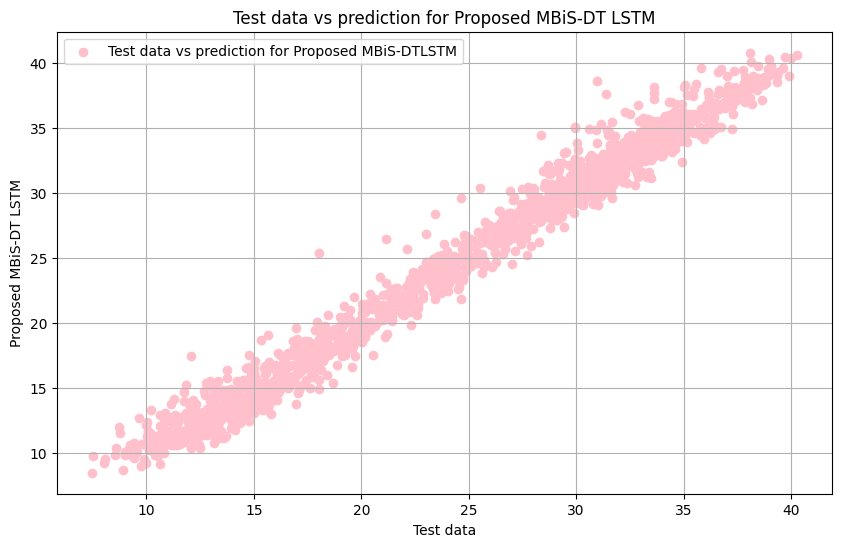
\includegraphics[scale=0.3]{scatter_lstm.png}\label{fig:ScatterPlot_TestDataVSMBiS-DT_LSTM}}
% \caption{Superimposed Prediction Scattered plot of traditional DL and proposed model over test data.}
% \label{fig:Scatter plot of vs proposed MBiS-DT models}
% \end{figure}




% \begin{figure}[ht!]
% \centering
% 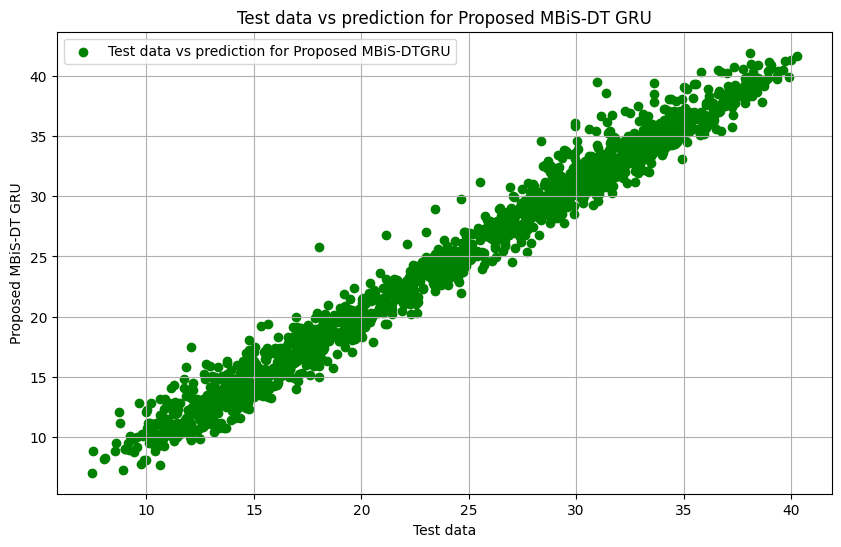
\includegraphics[width=1\textwidth, height=0.9\linewidth]{scatter_gru.png}
% \caption{Test data vs Proposed MBiS-DT GRU}
% \label{fig:ScatterPlot_TestDataVSMBiS-DT_GRU}
% \end{figure}
% \begin{figure}[ht!]
% \centering
% 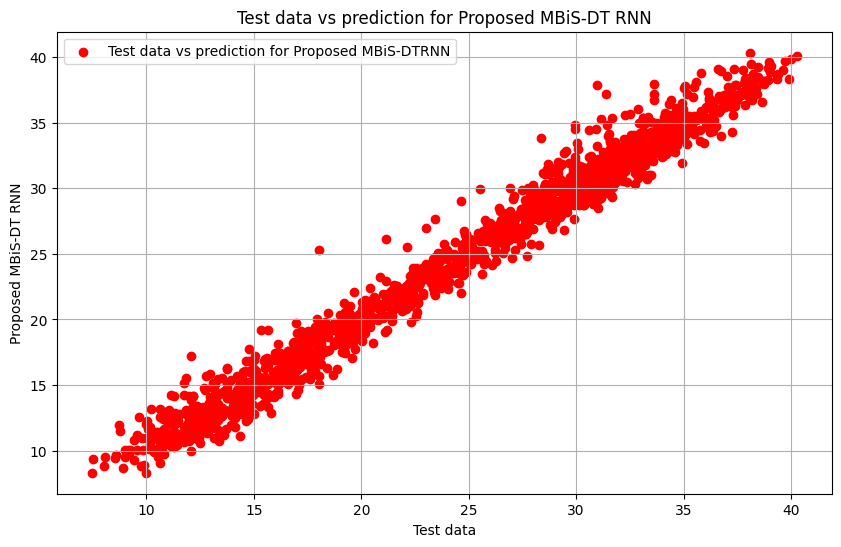
\includegraphics[width=1\textwidth, height=0.9\linewidth]{scatter_rnn.png}
% \caption{Test data vs Proposed MBiS-DT RNN}
% \label{fig:ScatterPlot_TestDataVSMBiS-DT_RNN}
% \end{figure}
% \begin{figure}[ht!]
% \centering
% 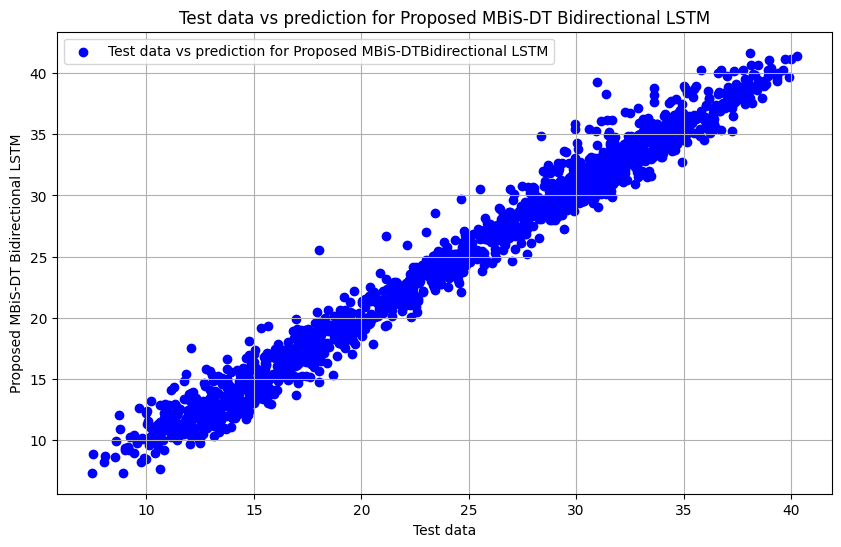
\includegraphics[width=1\textwidth, height=0.9\linewidth]{scatter_bilstm.png}
% \caption{Test data vs Proposed MBiS-DT BI-LSTM}
% \label{fig:ScatterPlot_TestDataVSMBiS-DT_BI-LSTM}
% \end{figure}
% \begin{figure}[ht!]
% \centering
% 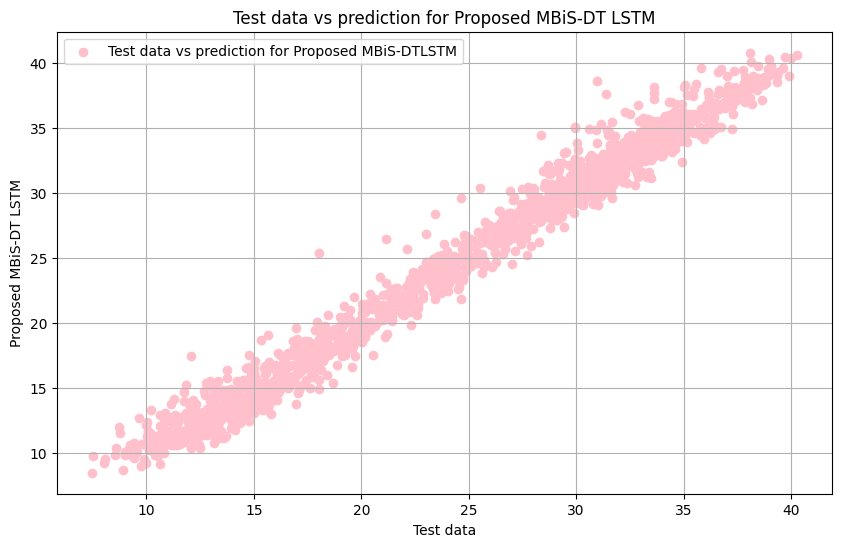
\includegraphics[width=1\textwidth, height=0.9\linewidth]{scatter_lstm.png}
% \caption{Test data vs Proposed MBiS-DT LSTM}
% \label{fig:ScatterPlot_TestDataVSMBiS-DT_LSTM}
% \end{figure}




\section{Performance Measures:}
\subsection{Root Mean Squared Error (RMSE):}
This performance metric is used widely in regression tasks, including temperature prediction. It calculates the average magnitude of the errors between actual and predicted values. The RMSE is calculated by taking the square root of the average of the squared differences between actual and predicted values.

The formula for RMSE is as in eqn. (\ref{eqn:e}):
\begin{equation}
\label{eqn:e}
RMSE = \sqrt {\frac{1}{N} \sum_{i=1}^{N} (\hat{y_{i}} - y_{i})^2}
\end{equation}
where the variables $\hat{y}_i$ is predicted values of the target variable (e.g., temperature), $y_i$ is the actual values of the target variable, and N is the total number of data point in the dataset.
\subsection{Mean Absolute Error (MAE):} It is a data-dependent performance metric used to evaluate the average exact error between actual and predicted variables. The formula for MAE is depicted in eqn. (\ref{eqn:mae})
\begin{equation}
\label{eqn:mae}
MAE = \frac{1}{N} \sum_{i=1}^{N} \left|\hat{y_{i}} - y_{i}\right| .
\end{equation}
where the variables $\hat{y}_i$ are predicted values of the target variable (e.g., temperature), $y_i$ are the actual values of the target variable, and N is the total no. of the data point in the dataset.

\subsection{Mean Squared Error (MSE):}
Mean Squared Error (MSE) is another widely used performance metric in regression tasks, including temperature prediction. It computes the Mean of the squared differences between actual and predicted values. MSE emphasizes a more significant error value than a more minor error value due to the squaring of the differences.
The formula for MSE is as depicted in eqn. (\ref{eqn:mse})
\begin{equation}
\label{eqn:mse}
MSE = \frac{1}{N} \sum_{i=1}^{N} (\hat{y_{i}} - y_{i})^2
\end{equation}
where the variables $\hat{y}_i$ are predicted values of the target variable (e.g., temperature), $y_i$ are the actual values of the target variable, and N is the number of data points in the dataset.


\subsection{Mean Absolute Percentage Error (MAPE):}
Mean Absolute Percentage Error (MAPE) is a performance metric commonly used in regression tasks, including temperature prediction. It measures the average percentage difference between predicted and actual values, providing a relative measure of the accuracy of the model's predictions.

The formula for MAPE is represented in eqn. (\ref{eqn:mape})
\begin{equation}
\label{eqn:mape}
MAPE = \frac{100}{N} \sum_{i=1}^{N} \left|(\frac{\hat{y_{i}} - y_{i}}{y_i})\right| .
\end{equation}

%MAPE = (1/n) * Σ(|(y_actual - y_pred) / y_actual|) * 100

where the variables $\hat{y}_i$ are predicted values of the target variable (e.g., temperature), $y_i$ are the actual values of the target variable, and N is the number of data points in the dataset.



\section{Implementation setup and parameters settings}
The various packages of Python are utilized to implement the baseline and proposed models. These include Pandas (v1.5.3), Scikit-Learn (v1.2.2) for model creation and performance analysis, Keras (v2.12.0), TensorFlow (v2.12.0) for Keras backend, and NumPy (v1.23.5) for exploratory data analysis, and For describing the findings and creating graphs, we used Plotly (v5.14.1), seaborn (v0.12.2), and Matplotlib (v3.7.1). To create flowcharts, it has also used \href{https://docs.google.com/drawings/}{https://docs.google.com/drawings/}. One system was employed for the experiments: a MacOS-based computer with Apple M1 having 8 GB RAM. All experiments were done on Google Colab with runtime Python 3 and hardware-accelerated T4 GPU with 12.7 GB RAM. Table \ref{tab: my-table} has the parameter values of the traditional DL and proposed models.

\begin{table*}[h!]
\centering
\setlength{\tabcolsep}{3pt}
{\renewcommand{\arraystretch}{1}%

\caption{Parameter setting of traditional DL models and proposed MBiS-DT Models}
\label{tab: my-table}
\begin{tabular}{ll}
\hline Hyperparameters & Values \\ \hline
Batch Size & 32 \\
Optimizer & Adam \\
Loss function & Mean Squared Error \\
Epoch & 200 with early stopping \\
training size & 0.8 \\ \hline
\end{tabular}}
\end{table*}
Upward batch and Downward batch ensemble(UD-Batch) and Corresponding upward and downward ensemble(CUD-ensemble)


%% Chapter Template

\chapter{Results and Analysis} % Main chapter title

\label{c5} % Change X to a consecutive number; for referencing this chapter elsewhere, use \ref{ChapterX}


\section{Results and Analysis}

\subsection{Quantitative Analysis}



\begin{table}[!p]
    \setlength{\tabcolsep}{3pt}
 {\renewcommand{\arraystretch}{1}%
    \caption{Performances of traditional DL models and both proposed models(i.e,  GRU-CNN(proposed-1)) and RB-GRU-CNN(proposed-2)) based on RMSE,  MSE,  MAE and MAPE measures over PTB diagnostic ECG datasets.}
    \label{tab:error_metrics}
    \begin{tabular}{p{0.08\linewidth}cccccccc}
        \toprule
        Error Metric & Dataset & CNN & RNN & LSTM & GRU & BiLSTM & PRO-1 & PRO-2 \\
        \midrule
        \multirow{9}{*}{RMSE} \\
        & D1 & 0.02511 & 0.029045 & 0.02845 & 0.023255 & 0.026725 & 0.017375 & 0.017246 \\
        & D2 & 0.048335 & 0.05851 & 0.033775 & 0.044645 & 0.054565 & 0.016211 & 0.01425 \\
        & D3 & 0.07086 & 0.07155 & 0.07388 & 0.069305 & 0.08139 & 0.04781 & 0.04211\\
        & D4 & 0.053515 & 0.05766 & 0.054275 & 0.051595 & 0.05713 & 0.048195 & 0.040361\\
        & D5 & 0.04291 & 0.02836 & 0.02967 & 0.07155 & 0.07086 & 0.02017 & 0.02\\
        & Mean & 0.048146 & 0.049025 & 0.04401 & 0.05207 & 0.058134 & 0.0299522 & 0.0267934 \\
        \midrule
        \multirow{9}{*}{MSE}\\
        & D1 & 0.000625 & 0.000905 & 0.00085 & 0.000555 & 0.00074 & 0.000315 & 0.000286 \\
        & D2 & 0.00236 & 0.003575 & 0.00118 & 0.002035 & 0.006135 & 0.000315 & 0.00029\\
        & D3 & 0.00505  & 0.00577 & 0.005465 & 0.00483 & 0.00662 & 0.002345 & 0.00219 \\
        & D4 & 0.002925 & 0.00359 & 0.002965 & 0.002685 & 0.00328 & 0.002335 & 0.00202 \\
        & D5 & 0.00204 & 0.00082 & 0.00089 & 0.00577 & 0.00505 & 0.00042 & 0.00031 \\
        & Mean & 0.0026 & 0.002932 & 0.00227 & 0.003175 & 0.004365 & 0.001146 & 0.0010192 \\
        \midrule
        \multirow{9}{*}{MAE}\\
        & D1 & 0.011715 & 0.01838 & 0.01557 & 0.012045 & 0.01579 & 0.00956 & 0.00852 \\
        & D2 & 0.03676 & 0.04618 & 0.01851 & 0.03445 & 0.0415 & 0.00811 & 0.0072 \\
        & D3 & 0.04694 & 0.044345 & 0.048095 & 0.043585 & 0.0491 & 0.03033 & 0.02318 \\
        & D4 & 0.035295 & 0.03525 & 0.03449 & 0.032885 & 0.034545 & 0.03131 & 0.02336 \\
        & D5  & 0.02873 & 0.018095 & 0.018915 & 0.044345 & 0.04694 & 0.011685 & 0.0045 \\
        & Mean & 0.031888 & 0.03245 & 0.027116 & 0.033462 & 0.037575 & 0.018199 & 0.013352 \\
        \midrule
        \multirow{9}{*}{MAPE}\\
        & D1 & 5.758535 & 9.3428 & 7.472155 & 5.433125 & 7.69268 & 4.65592 & 3.22098 \\
        & D2 & 6.144505 & 7.40371 & 9.10457 & 5.852235 & 6.849115 & 3.82211 & 3.2145 \\
        & D3 & 9.79425 & 10.242305 & 9.93871 & 9.85453 & 10.8904 & 5.962575 & 4.376 \\
        & D4 & 8.24417 & 9.73791 & 8.29686 & 8.59091 & 9.001425 & 6.950645 & 4.2018 \\
        & D5 & 4.98369 & 8.88995 & 5.698585 & 10.242305 & 9.79425 & 3.14022 & 3.11067 \\
        & Mean & 6.98503 & 9.123335 & 8.102176 & 7.994621 & 8.845574 & 4.906294 & 3.62479 \\
       
        \bottomrule
    \end{tabular}}
\end{table}

\begin{table}[!h]
\setlength{\tabcolsep}{3pt}
 {\renewcommand{\arraystretch}{1}%
    \caption{Percentage improvement over traditional models based on proposed-1 GRU-CNN model for RMSE,  MSE,  MAE and MAPE measures.}
    \label{tab:error_metrics}
    \begin{tabular}{ccccccc}
        \toprule
        Error Metric & Dataset & \%imp CNN & \%imp RNN & \%imp LSTM & 
        \%imp GRU & \%imp BiLSTM \\
        \midrule
        \multirow{7}{*}{RMSE} \\
        & D1 & 30.80\% & 40.17\% & 38.92\% & 25.28\% & 34.98\% \\
        & D2 & 66.46\% & 72.29\% & 52\% & 52\% & 70.29\% \\
        & D3 & 32.52\% & 33.17\% & 35.28\% & 31.01\% & 41.25\% \\
        & D4 & 9.94\% & 16.41\% & 11.20\% & 6.58\% & 15.63\%\\
        & D5 & 52.99\% & 28.87\% & 32\% & 71.80\% & 71.53\%\\
        & Mean & 38.54\% & 38.18\% & 33.88\% & 37.33\% & 46.74\%\\
        \midrule
        \multirow{7}{*}{MSE}\\
        & D1 & 49.60\% & 65.19\% & 62.94\% & 43.24\% & 57.43\%\\
        & D2 & 86.65\% & 91.18\% & 73.30\% & 84.52\% & 94.86\%\\
        & D3 & 53.56\%  & 59.35\% & 57.09\% & 51.44\% & 64.57\%\\
        & D4 & 20.17\% & 34.95\% & 21.24\% & 13.03\% & 28.81\%\\
        & D5 & 79.41\% & 48.78\% & 52.80\% & 92.72\% & 91.63\%\\
        & Mean & 57.88\% & 59.89\% & 53.47\% & 56.99\% & 67.46\%\\
        \midrule
        \multirow{7}{*}{MAE}\\
        & D1 & 18.39\% & 47.98\% & 38.59\% & 20.63\% & 39.45\%\\
        & D2 & 77.93\% & 82.43\% & 56.18\% & 76.45\% & 80.45\%\\
        & D3 & 35.38\% & 31.60\% & 36.93\% & 30.41\% & 38.22\%\\
        & D4 & 11.29\% & 11.17\% & 9.22\% & 4.78\% & 9.36\%\\
        & D5  & 59.32\% & 35.42\% & 38.22\% & 73.64\% & 75.10\%\\
        & Mean & 40.46\% & 41.72\% & 35.83\% & 41.18\% & 48.52\%\\
        \midrule
        \multirow{7}{*}{MAPE}\\
        & D1 & 19.14\% & 50.16\% & 37.68\% & 14.30\% & 39.47\%\\
        & D2 & 37.79\% & 48.37\% & 58.01\% & 34.68\% & 44.19\%\\
        & D3 & 39.12\% & 41.78\% & 40\% & 39.49\% & 45.24\%\\
        & D4 & 15.69\% & 28.62\% & 16.22\% & 19.09\% & 22.78\%\\
        & D5 & 36.99\% & 64.67\% & 44.89\% & 69.34\% & 67.93\%\\
        & Mean & 29.75\% & 46.72\% & 39.36\% & 35.38\% & 43.92\%\\ 
        \bottomrule
    \end{tabular}}
\end{table}  

It can be seen in Table 1 that on taking four performance metrics the 5 datasets when fed to traditional DL models and compared with proposed-1,  turns out proposed-1 is outperforming implemented traditional models. Proposed-1 is giving least RMSE compared to traditional DL models. Proposed-1(GRU-CNN) on all 5 datasets gave a mean value of RMSE 0.0299522 . A major \% improvement in proposed-1 with respect to traditional DL models can be seen in Table 2 where models CNN,  RNN,  LSTM,  GRU and BiLSTM shown a percentage improvement of 38.54\%,  38.18\%,  33.88\%,  37.33\% and 46.74\% respectively,  which are mean values of \% improvement in RMSE corresponding to datasets with respect to proposed-1 model. Quantitatively proposed-2 is giving less RMSE than proposed-1,  for the model proposed-2 on all 5 datasets a mean value of RMSE 0.0267934 is achieved hence,  it can be concluded that proposed-2 is better than proposed-1 since RMSE of proposed-2 is less than RMSE of proposed-1. 

Similarly,  from Table 1, it can be observed that  Proposed-1 is giving least MSE compared to traditional DL models. Proposed-1 on all 5 datasets gave a mean value of MSE 0.001146 . A major \% improvement in proposed-1 with respect to traditional DL models can be seen in Table 2 where models CNN,  RNN,  LSTM,  GRU and BiLSTM shown a percentage improvement of 57.88\%,  59.89\%,  53.47\%,  56.99\% and 67.46\% respectively,  which are mean values of \% improvement in MSE corresponding to datasets with respect to proposed-1 model. Quantitatively proposed-2 is giving less MSE than proposed-1,  for the model proposed-2 on all 5 datasets a mean value of MSE 0.0010192 is achieved hence,  it can be concluded that proposed-2 is better than proposed-1 since,  MSE of proposed-2 is less than MSE of proposed-1. 

Again,  from Table 1 it can be observed that  Proposed-1 is giving least MAE compared to traditional DL models. Proposed-1 on all 5 datasets gave a mean value of MAE 0.018199 . A major \% improvement in proposed-1 with respect to traditional DL models can be seen in Table 2 where models CNN,  RNN,  LSTM,  GRU and BiLSTM shown a percentage improvement of 40.46\%,  41.72\%,  35.83\%,  41.18\% and 48.52\% respectively,  which are mean values of \% improvement in MAE corresponding to datasets with respect to proposed-1 model. Quantitatively proposed-2 is giving less MAE than proposed-1,  for the model proposed-2 on all 5 datasets a mean value of MAE 0.013352 is achieved Hence,  it can be concluded that proposed-2 is better than proposed-1 since MAE of proposed-2 is less than MAE of proposed-1.

At last,  from Table 1 it can be observed that  Proposed-1 is giving least MAPE compared to traditional DL models. Proposed-1 on all 5 datasets gave a mean value of MAPE 4.906294 . A major \% improvement in proposed-1 with respect to traditional DL models can be seen in Table 2 where models CNN,  RNN,  LSTM,  GRU and BiLSTM shown a percentage improvement of 29.75\%,  46.72\%,  39.36\%,  35.38\% and 43.92\% respectively,  which are mean values of \% improvement in MAPE corresponding to datasets with respect to proposed-1 model. Quantitatively proposed-2 is giving less MAPE than proposed-1,  for the model proposed-2 on all 5 datasets a mean value of MAPE 3.62479 is achieved hence,  it can be concluded that proposed-2 is better than proposed-1 since MAPE of proposed-2 is less than MAPE of proposed-1.
 \begin{figure*}[h!]
   \centering
   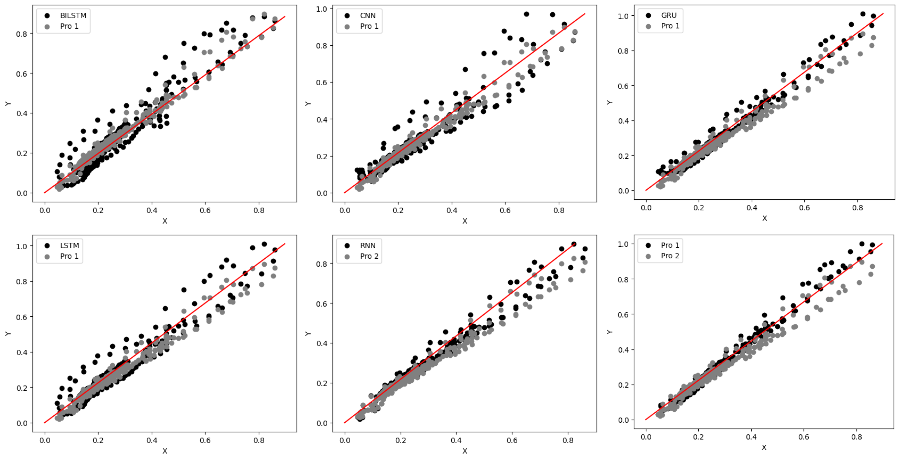
\includegraphics[scale=.5]{d1_sp.drawio.png}
     %\captionsetup{justification=centering, margin=2cm}
    \caption{Scatter plots of proposed GRU-CNN(pro-1) with stand alone DL models along with proposed-2 RB-GRU-CNN(pro-2), where x-axis \& y-axis represent the predictions of models and original test data D1.}
    \label{Fig:6}
   \end{figure*}
   \begin{figure*}[h!]
    \centering
     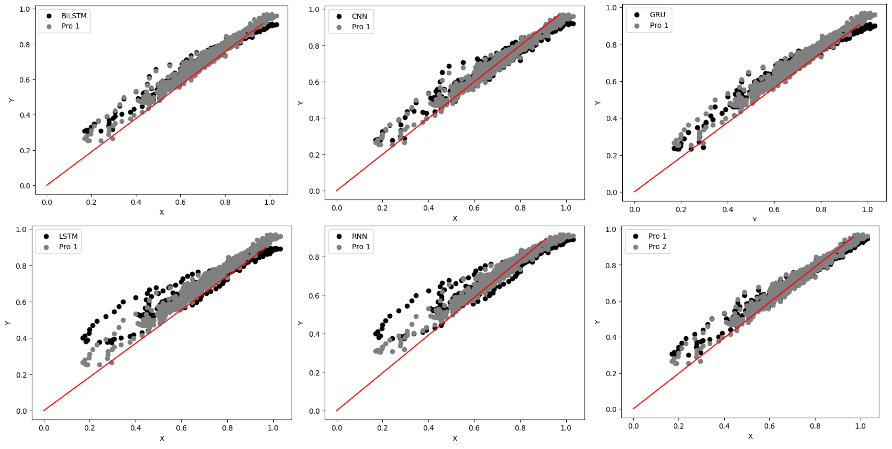
\includegraphics[scale=.5]{d2_sp.drawio.png}
     \caption{Scatter plots of proposed GRU-CNN(pro-1) with stand alone DL models along with proposed-2 RB-GRU-CNN(pro-2), where x-axis \& y-axis represent the predictions of models and original test data D2.}
     \label{Fig:7}
  \end{figure*}
  \begin{figure*}[h!]
     \centering
     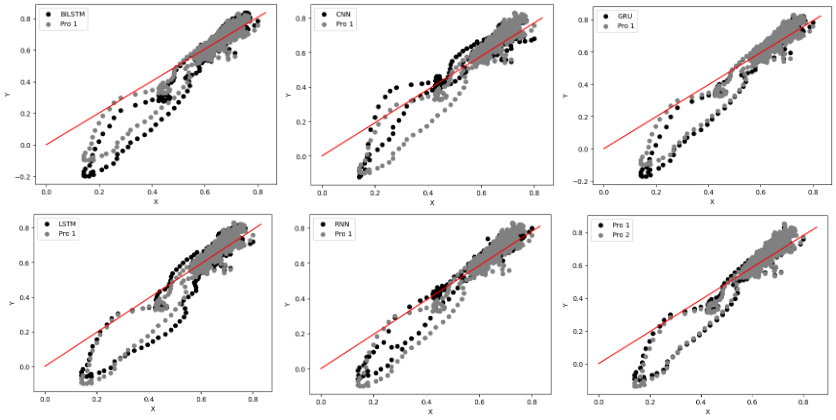
\includegraphics[scale=.5]{d3_sp.drawio.png}
     \caption{Scatter plots of proposed GRU-CNN(pro-1) with stand alone DL models along with proposed-2 RB-GRU-CNN(pro-2), where x-axis \& y-axis represent the predictions of models and original test data D3.}
     \label{Fig:8}
   \end{figure*}
   \begin{figure*}[h!]
    \centering
     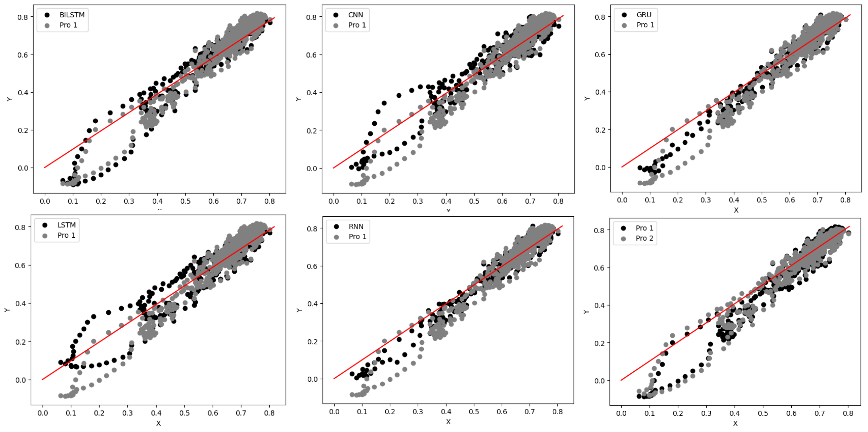
\includegraphics[scale=.5]{d4_sp.drawio.png}
     \caption{Scatter plots of proposed GRU-CNN(pro-1) with stand alone DL models along with proposed-2 RB-GRU-CNN(pro-2), where x-axis \& y-axis represent the predictions of models and original test data D4.}
     \label{Fig:9}
   \end{figure*}
   \begin{figure}[h!]
    \centering
     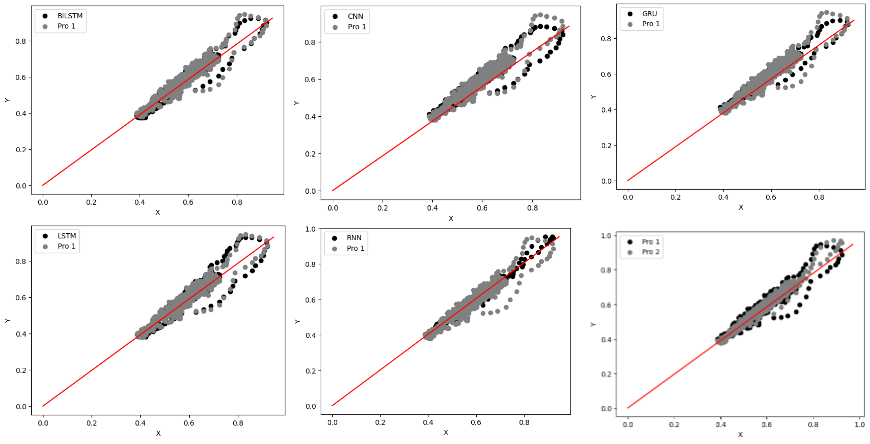
\includegraphics[scale=.5]{d5_sp.drawio.png}
     \caption{Scatter plots of proposed GRU-CNN(pro-1) with stand alone DL models along with proposed-2 RB-GRU-CNN(pro-2), where x-axis \& y-axis represent the predictions of models and original test data D5.}
     \label{Fig:10}
   \end{figure}

   \begin{figure*}[h!]
    \centering
     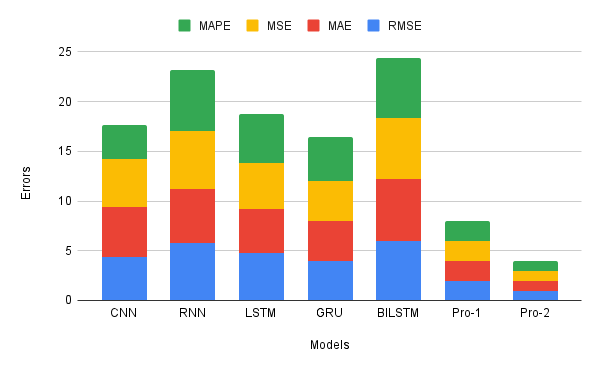
\includegraphics[scale=.6]{aggregator.png}
     \caption{Aggregate measures comparison of traditional models and proposed (pro-1 \& pro-2) models.}
     \label{Fig:13}
   \end{figure*} 
\subsection{Graphical Analysis}
 \begin{figure*}[h!]
    \centering
    \subfigure{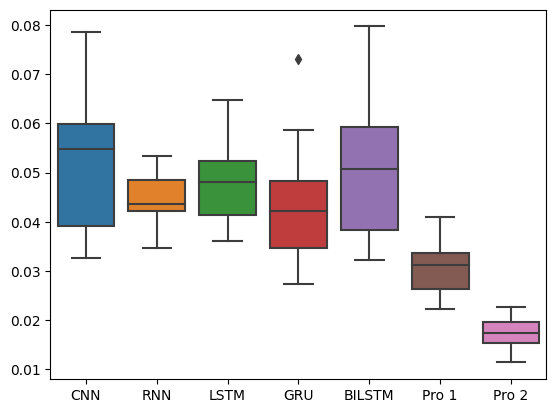
\includegraphics[scale=0.5]{d1rmse}}
    \subfigure{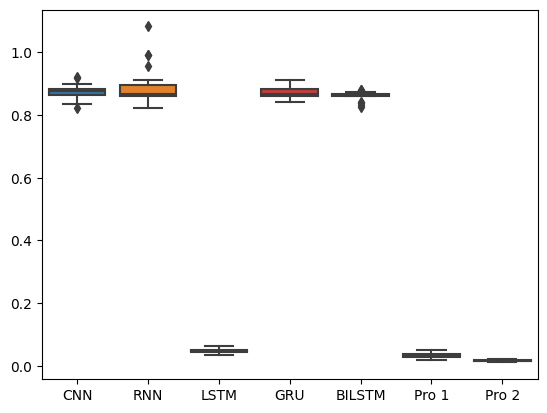
\includegraphics[scale=0.5]{D2_RMSE}}
    \subfigure{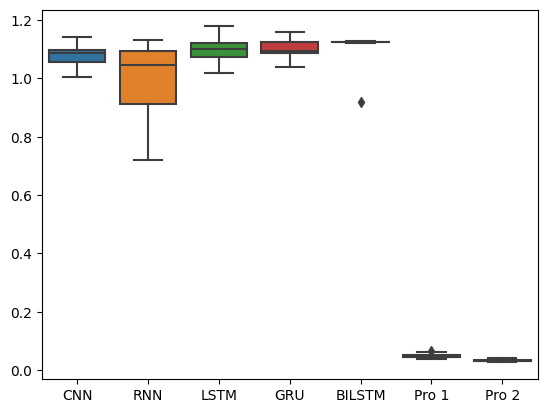
\includegraphics[scale=0.5]{D3_RMSE}}
    \subfigure{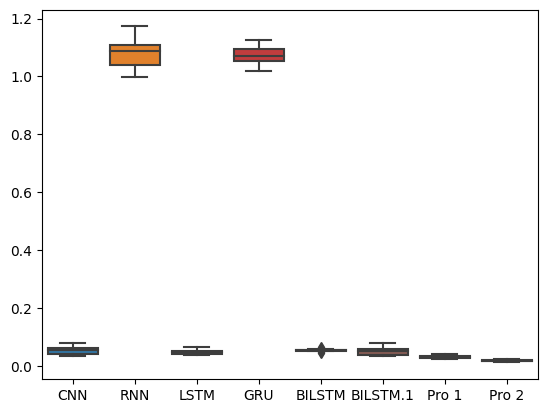
\includegraphics[scale=0.5]{d4_rmse}}
    \subfigure{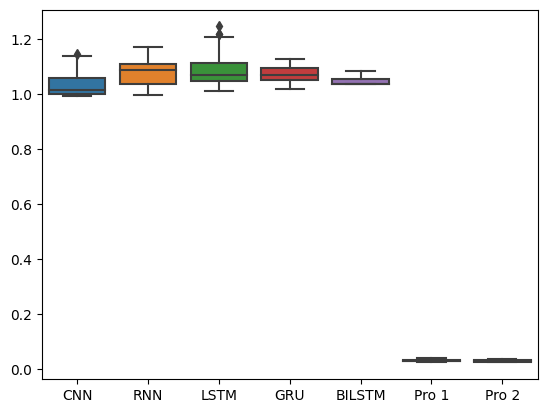
\includegraphics[scale=0.5]{D5_RMSE}}
    \caption{RMSE (performance box-plots) of basic DL models with proposed hybrid models (pro-1 \& pro-2).}
    \label{Fig:14}
  \end{figure*}

  \begin{figure*}[h!]
    \centering
    \subfigure{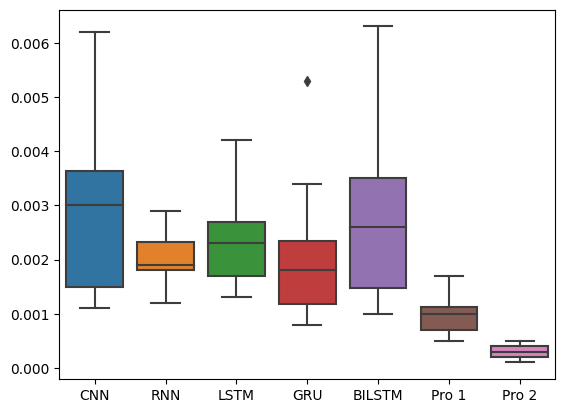
\includegraphics[scale=0.5]{d1_mse}}
    \subfigure{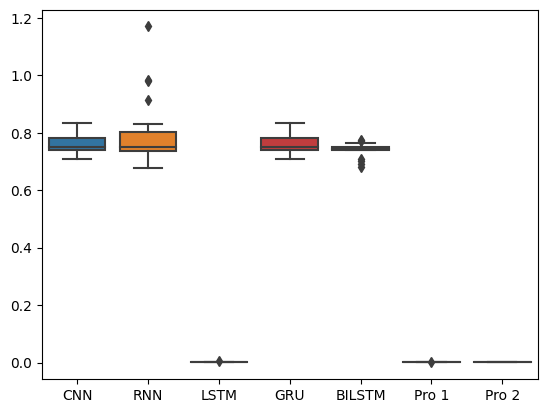
\includegraphics[scale=0.5]{D2_MSE}}
    \subfigure{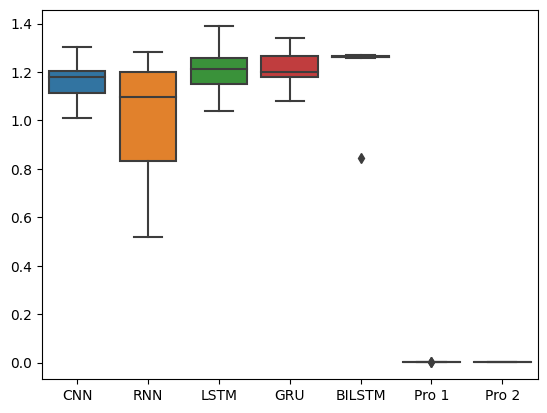
\includegraphics[scale=0.5]{D3_MSE}}
    \subfigure{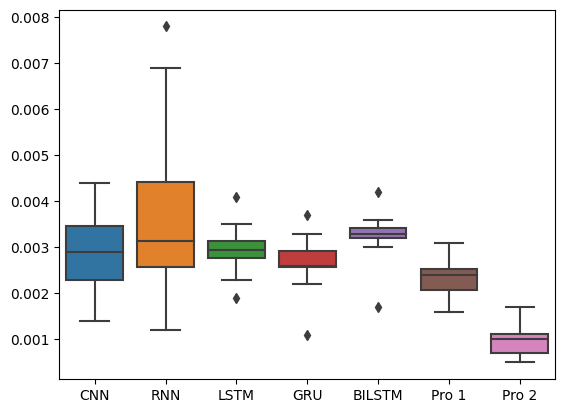
\includegraphics[scale=0.5]{d4_mse}}
    \subfigure{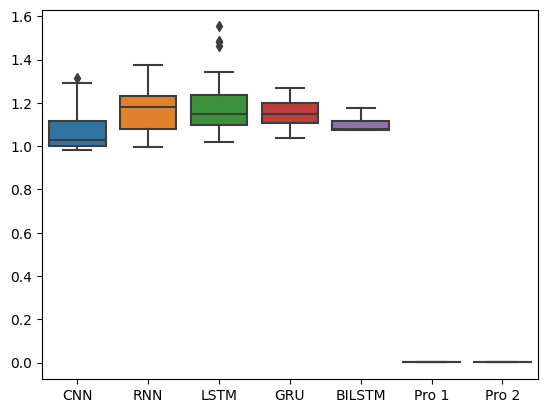
\includegraphics[scale=0.5]{D5_MSE}}
    \caption{MSE (performance box-plots) of basic DL models with proposed hybrid models (pro-1 \& pro-2).}
    \label{Fig:15}
  \end{figure*}

  \begin{figure*}[h!]
   \centering
    \subfigure{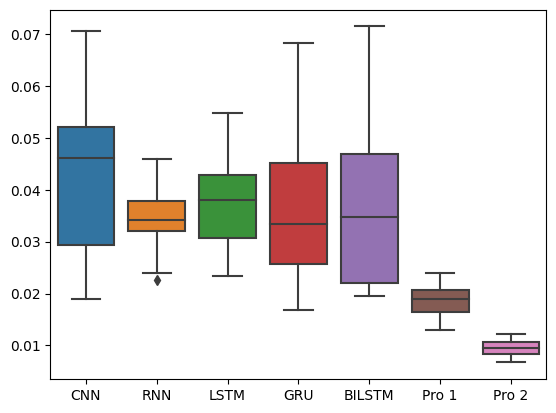
\includegraphics[scale=0.5]{d1_mae}} 
    \subfigure{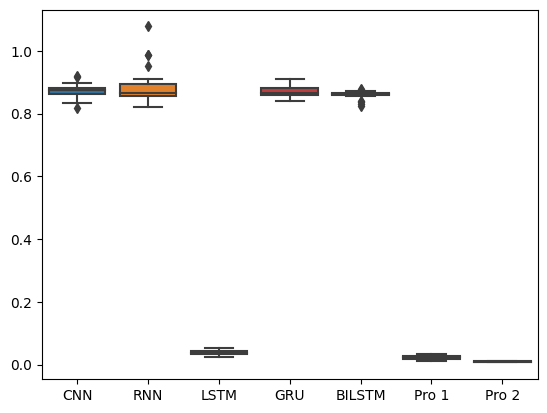
\includegraphics[scale=0.5]{D2_MAE}}
    \subfigure{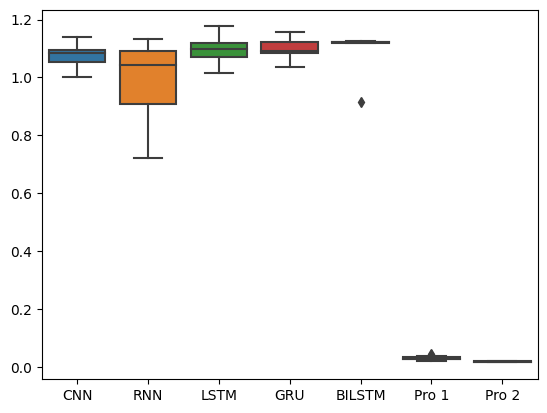
\includegraphics[scale=0.5]{D3_MAE}}
    \subfigure{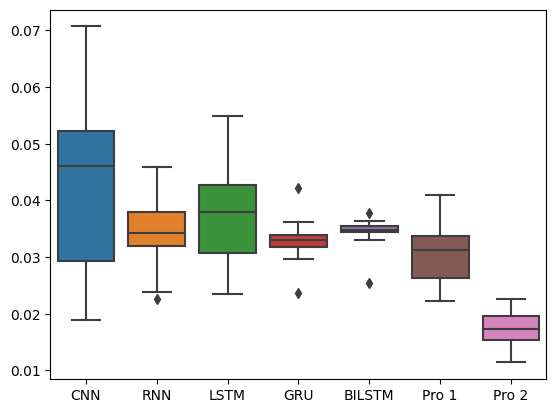
\includegraphics[scale=0.5]{d4_mae}}
    \subfigure{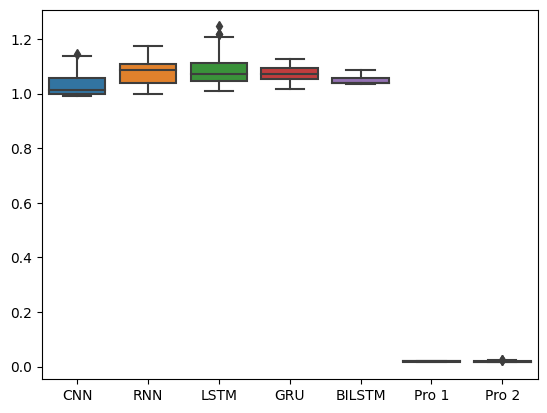
\includegraphics[scale=0.5]{D5_MAE}}
    \caption{MAE (performance box-plots) of basic DL models with proposed hybrid models (pro-1 \& pro-2).}
    \label{Fig:16}
  \end{figure*}
  \begin{figure*}[h!]
    \centering
    \subfigure{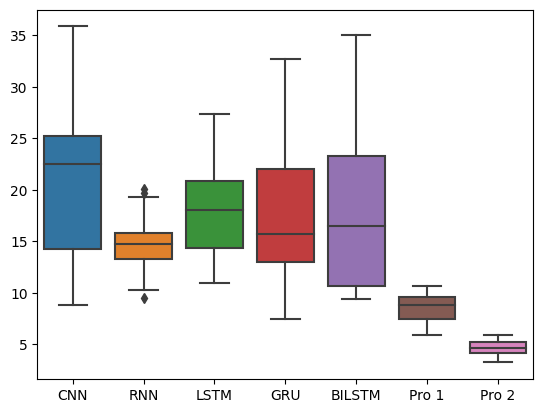
\includegraphics[scale=0.5]{d1_mape}}
    \subfigure{\includegraphics[scale=0.5]{D2_MAPE}}
    \subfigure{\includegraphics[scale=0.5]{D3_MAPE}}
    \subfigure{\includegraphics[scale=0.5]{d4_mape}} 
    \subfigure{\includegraphics[scale=0.5]{D5_MAPE}}
    \caption{MAPE (performance box-plots) of basic DL models with proposed hybrid models (pro-1 \& pro-2).}
    \label{Fig:17}
  \end{figure*}
In this section graphical analysis of our experiments is shown. Overlaying the scatterplot is a line of regression with a distinct 45-degree angle. The angle indicates that there is a high positive correlation between the two variables,  implying a linear relationship. Two more regression lines are visible on the scatterplot upon closer scrutiny. One of these lines closely follows the general trend of the data points,  with a relatively limited deviation off the line. This indicates a good fit for the data and a high prediction power for the model it represents. Although it still follows the main trend,  the other regression line deviates further from the scatterplot's points. This line clearly has a larger range of data points surrounding it. This indicates a poorer fit than the first model. When the two models are compared,  it is evident that the first,  with its narrower spread and greater alignment to the data points,  produces more accurate results. In Figure 8 on dataset D1 proposed-1(pro-1) can be seen scattered and overlapping the traditional DL models and in the last figure proposed-2 is overlapping proposed-1 validating proposed-1 to be outperforming traditional DL models and proposed-2(pro-2) is better than proposed-1. Similarly,  it can be understood for Figure 9,  10,  11 and 12 where predicted dataset belongs to D2,  D3,  D4 and D5. Boxplot has the ability to obtain insights into the distribution of numerical data,  it is one of the best ways to undertake statistical analysis since it gives a compact approach to visualise the spread,  central tendency,  and probable outliers. It can be seen from the plot in Figure 14 all five datasets are analysed on the basis of RMSE,  where traditional models are compared with proposed-1 and proposed-2. Here proposed-2 is better than proposed-1 and traditional DL models are outperformed by the proposed ones. Similarly,  in Figure 15 all five datasets are analysed on the basis of MSE and comparative analysis has outperformed the traditional DL models,  with proposed-2 is better than proposed-1. Again in Figure 16 a comparative analysis on the basis of MAE is observed corresponding to all five datasets,  where proposed-2 is working better than proposed-1 and outperforming the traditional DL models. At last in Figure 17 it can be observed,  analysis of traditional DL models is performed corresponding to five datasets with proposed-1 and proposed-2 on taking MAPE the metric,  where proposed-2 is seen to be working better than proposed-1 and proposed-1 outperforming the rest of the traditional DL models. A summarised analysis can be understood by plot Figure 13 that shows all performance metric to be averaged and plotted against the traditional and proposed models. It can be concluded from the figure that pro-1(proposed-1) is giving minimum error compared to traditional DL models and pro-2(proposed-2) is giving less error than proposed-1 hence, the best among all.
 

\subsection{Statistical Analysis}

In this section Friedman test is used to validate proposed-1 and proposed-2  are better performing models than traditional DL models on the basis of rank,  p-value and holm. A non-parametric statistical test is performed on RMSE,  MSE,  MAE and MAPE achieved by taking the mean of results achieved after 20 iterations of every single model. Table 3 shows non-parametric test results where it can be seen that our proposed-2 giving rank 1 on all the performance measures while,  proposed-1 came to be following rank 2. The null hypothesis is rejected for proposed-1 because of its p-value 0.464214 which is greater than  $\alpha = 0.05$ , 
 which means proposed-1 and proposed-2 have similar performance. However,  based on holm’s procedure the hypothesis of proposed-1 is rejected because its holm’s value is 0.05,  which is equal to hypothesis value. Therefore,  it can be said that the proposed-1 and proposed-2 models are distinct based on holm’s procedure. The values and Ranking are as follows Figure 18:

\begin{figure*}[ht!]
  \centering
   \includegraphics[scale=.7]{rankplot.png}
   \caption{Overall ranking of Traditional models \& Proposed models corresponding to all performance measures.}
 \end{figure*}

\begin{table}[htbp]
\centering
    \setlength{\tabcolsep}{3pt}
 {\renewcommand{\arraystretch}{1}%
    \caption{Non-parametric statistical analysis via Friedman ranking,  p-value \& Holm's procedure over various performance measure as RMSE,  MSE,  MAE and MAPE.}
    \begin{tabular}{cccccc}
        \toprule
        Error Metric & Models & RANK & P-value & Holm \\
        \midrule
        \multirow{5}{*}{RMSE} & CNN & 4.4 & \textbf{0.012827} & \textbf{0.016667} \\
        & RNN & 5.8 & \textbf{0.000443} & \textbf{0.01} \\
        & LSTM & 4.8 & \textbf{0.005414} & \textbf{0.0125} \\
        & GRU & 4 & \textbf{0.028108} & \textbf{0.025} \\
        & BiLSTM & 6 & \textbf{0.000253} & \textbf{0.008333} \\
        & Pro-1 & 2  & 0.464214 & 0.05\\
        & Pro-2 & \textbf{1}  & - & -\\
        \midrule
        \multirow{5}{*}{MSE} & CNN & 4.4 & \textbf{0.012827} & \textbf{0.016667} \\
        & RNN & 5.8 & \textbf{0.000443} & \textbf{0.01} \\
        & LSTM & 4.6 & \textbf{0.008415} & \textbf{0.0125} \\
        & GRU & 4 & \textbf{0.028108} & \textbf{0.025} \\
        & BiLSTM & 6.2 & \textbf{0.000141} & \textbf{0.008333} \\
        & Pro-1 & 2 & 0.464214 & 0.05 \\
        & Pro-2 & \textbf{1}  & - & -\\
        \midrule
        \multirow{5}{*}{MAE} & CNN & 5 & \textbf{0.003415} & \textbf{0.0125} \\
        & RNN & 5.4 & \textbf{0.00128} & \textbf{0.01} \\
        & LSTM & 4.4 & \textbf{0.012827} & \textbf{0.016667} \\
        & GRU & 4 & \textbf{0.028108} & \textbf{0.025} \\
        & BiLSTM & 6.2 & \textbf{0.000141} & \textbf{0.008333} \\
        & Pro-1 & 2 & 0.464214 & 0.05 \\
        & Pro-2 & \textbf{1}  & - & -\\
        \midrule
        \multirow{5}{*}{MAPE} & CNN & 3.4 & \textbf{0.078983} & \textbf{0.025} \\
        & RNN & 6.2 & \textbf{0.000141} & \textbf{0.008333} \\
        & LSTM & 5 & \textbf{0.003415} & \textbf{0.0125} \\
        & GRU & 4.4 & \textbf{0.012827} & \textbf{0.016667} \\
        & BiLSTM & 6 & \textbf{0.000253} & \textbf{0.01} \\
        & Pro-1 & 2 & 0.464214 & 0.05 \\
        & Pro-2 & \textbf{1}  & - & -\\
        \bottomrule
    \end{tabular}}
    
    \label{tab:error_metrics}
\end{table}

% Chapter Template

\chapter{Conclusion} % Main chapter title

\label{c6} % Change X to a consecutive number; for referencing this chapter elsewhere, use \ref{ChapterX}

\section{Conclusion}
Traditional DL models are implemented in this research by feeding PTB diagnostic ECG datasets from 5 different patients. These datasets are subjected to a time series analysis. A GRU-CNN hybrid model is constructed which is called proposed-1 throughout the studies. It has been seen that proposed-1 is outperforming traditional DL models. The significance of our investigation is based on the data that was collected. Our datasets' distinguishing qualities are highlighted. This research could help with future analyses of the PTB Diagnostic ECG database. Since, ECG is a one-dimensional signal,  1-D CNN is employed without any additional processing. However,  because CNNs learning is heavily reliant on data,  uneven data or inaccurate data labels can easily lead CNN models astray. The RMSE, MSE, MAE \& MAPE is shown to be giving least error on proposed-1(GRU-CNN) in comparison to the rest of the traditional DL models. To improve the results another model RB-GRU-CNN is proposed which is called proposed-2 throughout the studies. Proposed-2 has performed better than proposd-1 hence,  it can be concluded that GRU-CNN is better than traditional DL models and RB-GRU-CNN is better than GRU-CNN. Experimental validation for our proposed-1 and proposed-2 is done by non-parametric statistical analysis called Friedman test. 

\subsection*{CRediT authorship contribution statement}

\textbf{S.Khan} : Conceptualization, methodology, formal analysis, Resource, Writing original draft, visualization.\\
\textbf{Vipin Kumar} : methodology, conceptualization, validation, investigation, writing, review editing, supervision.

\subsection*{Data availability}



The data is available on the Physionet website. A full clinical summary is included in the header (.hea) file of the majority of these ECG records, including age, gender, diagnosis, and, when appropriate, data on medical history, medicines and treatment, coronary artery pathology, ventriculography, echocardiography, and hemodynamics. The clinical summary for 22 individuals is unavailable. This database has shown to be a valuable research resource for ECG investigations.





\subsection*{Acknowledgments}

A heartfelt applause to the Physionet's attempt in making this research possible by providing free clinical records to study cardiovascular diseases by people who have no prior idea about clinical sciences. 
% % Chapter Template

\chapter{Data availability \& Acknowledgement} % Main chapter title

\label{c7} % Change X to a consecutive number; for referencing this chapter elsewhere, use \ref{ChapterX}

%----------------------------------------------------------------------------------------
%	SECTION 1
%----------------------------------------------------------------------------------------
\section*{Data availability}
Data will be available on \href{https: //app.cpcbccr.com/ccr/#/caaqm-dashboard-all/caaqm-landing}{CPCB(India)} Webportel.The \href{https: //www.cpcb.nic.in/}{Central Pollution Control Board (CPCB) } in India maintains a web portal that offers access to various environmental datasets,  including air and water quality,  emission inventories,  and pollution monitoring data,  aimed at promoting environmental awareness and research in the country.

\section*{Acknowledgments}
We extend our heartfelt appreciation to the Central Pollution Control Board (CPCB),  India,  for generously providing invaluable environmental data,  which significantly enhanced our research and played a pivotal role in completing this study.

%\include{Chapters/Chapter1}
%\include{Chapters/Chapter2} 
%\include{Chapters/Chapter3}
%\include{Chapters/Chapter4}

%-----------------------appendix---------------------
%----------------------------------------------------------------------------------------
%	THESIS CONTENT - APPENDICES
%----------------------------------------------------------------------------------------

\appendix % Cue to tell LaTeX that the following "chapters" are Appendices

% Include the appendices of the thesis as separate files from the Appendices folder
% Uncomment the lines as you write the Appendices

%% Appendix A

\chapter{Frequently Asked Questions} % Main appendix title

\label{AppendixA} % For referencing this appendix elsewhere, use \ref{AppendixA}

\section{How do I change the colors of links?}

The color of links can be changed to your liking using:

{\small\verb!\hypersetup{urlcolor=red}!}, or

{\small\verb!\hypersetup{citecolor=green}!}, or

{\small\verb!\hypersetup{allcolor=blue}!}.

\noindent If you want to completely hide the links, you can use:

{\small\verb!\hypersetup{allcolors=.}!}, or even better: 

{\small\verb!\hypersetup{hidelinks}!}.

\noindent If you want to have obvious links in the PDF but not the printed text, use:

{\small\verb!\hypersetup{colorlinks=false}!}.

%\include{Appendices/AppendixB}
%\include{Appendices/AppendixC}

%-----------------------appendix---------------------

%----------------------------------------------------------------------------------------
%	BIBLIOGRAPHY
%----------------------------------------------------------------------------------------
%\documentclass{article}
\printbibliography[title={References},heading=bibintoc]
%\bibliographystyle{IEEEtran}
%\bibliography{Bibliography.bib}
%\end{document}
%----------------------------------------------------------------------------------------

%----------------------------------------------------------------------------------------
%--------------------cover----------------------
%%----------------------------------------------------------------------------------------
%	COVER PAGE
%----------------------------------------------------------------------------------------

\begin{titlepage}
\begin{center}

%\vspace*{.06\textheight}

%\textsc{\Large Masters Thesis}\\[0.5cm] % Thesis type

%\HRule \\[0.4cm] % Horizontal line
{\LARGE \bfseries \ReportTitel \par}\vspace{0.3cm} % Thesis title
%\HRule \\[1.5cm] % Horizontal line

%\begin{minipage}[t]{0.4\textwidth}
%\begin{flushleft} \large
%%\emph{Author:}\\
%%\href{http://www.johnsmith.com}{\authorname} % Author name - remove the \href bracket to remove the link
%\end{flushleft}
%\end{minipage}
%\begin{minipage}[t]{0.4\textwidth}
%\begin{flushright} \large
%%\emph{Supervisor:} \\
%%\href{http://www.jamessmith.com}{\supname} % Supervisor name - remove the \href bracket to remove the link
%\end{flushright}
%\end{minipage}\\[1cm]
%
\vfill

\large \textit{A \rType  submitted to the \Uni}\\[0cm] % University requirement text
\large \textit{in partially fulfillment of the requirements}\\[0cm]
\large \textit{for the award of the degree of}\\[0cm]

\textbf{\Degree}\\[0cm]

\uppercase{In}\\[0cm]

\uppercase{\textbf{\Cour}}\\[0cm]

\uppercase{By}\\[0cm]

\uppercase{\textbf{\fAuthorC}}\\[1cm]




%   \begin{figure}[H]
        %   \centering
\centerline{\includegraphics[height=1.5in,width=1.5in, keepaspectratio]{mgcu.png}}
        %   \includegraphics{logo}% logo
    %   \end{figure}
\vfill
\vspace{1cm}
\normalsize{\departmentC}\\[-0.1cm] %search group name and department name
%\school\\[0.1cm]
%\large{\groupname}\\[-0.2cm]

{\scshape\Large \UniversityC \par}\vspace{1cm} % University name%\university\\[2cm]
\vfill

{\large \today}\\[1cm] % Date
%\includegraphics{Logo} % University/department logo - uncomment to place it

\vfill

\end{center}
\end{titlepage}
%--------------------cover----------------------
\end{document}
